%
% chapter.tex -- Spezielle Funktionen definiert durch Integrale
%
% (c) 2021 Prof Dr Andreas Müller, Hochschule Rapperswil
%
% !TeX spellcheck = de_CH
\chapter{Integrale
\label{buch:chapter:integral}}
\lhead{Integrale}
\rhead{}
Der Analysis-Unterricht vermittelt manchmal den Eindruck, dass sich
für jede einigermassen anständige Funktion eine Stammfunktion
gefunden werden kann, wenn man nur genügend schlau ist und den 
nötigen Fleiss in die Lösung des Problems investiert.
Die Realität ist leider eine ganz andere, Ableiten ist zwar einfach,
eine Stammfunktion finden ist oft viel schwieriger und manchmal schlicht
unmöglich.

Der Ausweg aus dieser unangenehmen Situation ist, solche Integrale
als neue spezielle Funktionen zu definieren.
Eines der berühmtesten Beispiele für diesen Weg aus der Krise ist die
Fehlerfunktion, die im Abschnitt~\ref{buch:integrale:section:fehlerfunktion}
besprochen wird.
Auch geometrische Anwendungen führen auf solche Integrale.
Die Länge eines Ellipsenbogens kann mit Hilfe eines Integrals
berechnet werden, doch scheint es nicht möglich zu sein, für den
Umfang der Ellipse eine einfache Formel anzugeben, wie dies beim
Kreis möglich ist.
Dieses Problem führt auf eine ganze Familie von Integranden, die nicht in
geschlossener Form integriert werden können, nämlich die elliptischen
Funktionen.
Sie werden in Kapitel~\ref{buch:chapter:elliptischefunktionen} erklärt.

Doch wie entscheidet man, ob ein Integral tatsächlich nicht in geschlossener
Form dargestellt werden kann oder ob die Versuche einfach an mangelnden
eigenen Fähigkeiten gescheitert sind?
Denn warum soll man eine neue spezielle Funktion definieren, wenn es
dafür bereits eine gute Darstellung in geschlossener Form gibt?
Der Risch-Algorithmus von Abschnitt~\ref{buch:integral:section:risch}
gibt darauf eine Antwort.

%
% fehlerfunktion.tex
%
% (c) 2021 Prof Dr Andreas Müller, OST Ostschweizer Fachhochschule
%
\section{Die Fehlerfunktion
\label{buch:integrale:section:fehlerfunktion}}
\rhead{Fehlerfunktion}
Die Wahrscheinlichkeitsdichte einer normalverteilten Zufallsvariable $X$
mit Erwartungswert $\mu$ und Varianz $\sigma^2$ ist
\begin{equation}
\varphi(x)
=
\frac{1}{\sqrt{2\pi}\sigma}
e^{-\frac{(x-\mu)^2}{2\sigma^2}}.
\label{buch:integrale:eqn:normaldichte}
\end{equation}
Die Verteilungsfunktion der Zufallsvariable ist dann durch das Integral
\begin{equation}
f(x)
=
F_X(x)
=
P(X\le x)
=
\frac{1}{\sqrt{2\pi}\sigma}
\int_{-\infty}^x 
e^{-\frac{(t-\mu)^2}{2\sigma^2}}
\,dt
\label{buch:integrale:eqn:normalverteilung}
\end{equation}
gegeben.
Die Erfahrung zeigt, dass es nicht möglich ist, das
Integral~\eqref{buch:integral:eqn:normalverteilung}
in geschlossener Form auszuwerten.
Die Funktion $F_X(x)$ ist offenbar eine in Anwendungen nützliche und
häufig gebrauchte Funktion, die es verdient, in eine Standardbibliothek
von Funktion aufgenommen zu werden.
Dabei soll auch berücksichtigt werden, dass die neu zu definierende
spezielle Funktion möglichst auch für andere Anwendungen verwendet
werden kann, wie zum Beispiel die Berechnung gewisser Laplace-Transformierter.
Im Folgenden soll gezeigt werden, in welcher Form genau dies geschehen
kann.

%
% Vereinfachung des Integrals durch Standardisierung
%
\subsection{Standardisierung}
Die Formel~\ref{buch:integrale:eqn:normalverteilung} enthält die zwei 
Parameter $\mu$ und $\sigma$, sie ist daher als Basis für eine neue
spezielle Funktion nicht geeignet.
In diesem Abschnitt sollen sie eliminiert werden mit dem Ziel, ein
neues, einfacheres Integral zu definieren, aus dem sich 
\ref{buch:integrale:eqn:normalverteilung} leicht berechnen lässt.

\subsubsection{Elimination der Parameter $\mu$ und $\sigma$}
Aus der Wahrscheinlichkeitstheorie ist bekannt, dass zu einer
Zufallsvariablen $X$ mit Erwartungswert $E(X)=\mu$ und Varianz
$\operatorname{var}(X)=\sigma^2$ immer eine Zufallsvariable
gefunden werden kann mit Erwartungswert $0$ und Varianz $1$.
Tatsächlich bekommt man für die standardisierte Zufallsvariable
\begin{equation}
Z = \frac{X-\mu}{\sigma}
\label{buch:integrale:eqn:standardisierung}
\end{equation}
die Werte
\begin{align*}
E(Z)
&=
E\biggl(\frac{X-\mu}{\sigma}\biggr)
=
\frac{E(X)-\mu}{\sigma}
=
\frac{\mu-\mu}{\sigma}
=
0
\\
\text{und}\qquad
\operatorname{var}(Z)
&=
\operatorname{var}\biggl(\frac{X-\mu}{\sigma}\biggr)
=
\frac{\operatorname{var}(X)}{\sigma^2}
=
1,
\end{align*}
wie versprochen.
Dies bedeutet, dass sich das Integral~\ref{buch:integrale:eqn:normalverteilung}
durch ein Integral ausdrücken lassen muss, in der die Parameter $\mu$
und $\sigma$ nicht mehr vorkommen.

Die Standardisierungsformel~\eqref{buch:integrale:eqn:standardisierung}
deutet auch bereits an, wie man das
Integral~\ref{buch:integrale:eqn:normalverteilung} vereinfachen kann.
Dazu führen wir die Substitution $z=(t-\mu)/\sigma$ aus und erhalten
\begin{align*}
f(x)
&=
\frac{1}{\sqrt{2\pi}\sigma} 
\int_{-\infty}^x e^{-\frac{(t-\mu)^2}{2\sigma^2}}\,dt
=
\frac{1}{\sqrt{2\pi}\sigma}
\int_{\infty}^{(x-\mu)/\sigma}
e^{-\frac{z^2}2}\,\sigma dz
=
\frac{1}{\sqrt{2\pi}}
\int_{-\infty}^{\frac{x-\mu}{\sigma}} e^{-\frac{z^2}2}\,dz.
\end{align*}
Das Integral auf der rechten Seite enthält die Parameter $\mu$ und
$\sigma$ nur noch in der Integrationsgrenze.
Es kann durch die Wahrscheinlichkeitsverteilungsfunktion der
Standardnormalverteilung
\begin{equation}
\Phi(x) = \frac{1}{\sqrt{2\pi}} \int_{-\infty}^x e^{-\frac{z^2}2}\,dz
\label{buch:integrale:eqn:standardnormalverteilung}
\end{equation}
ausgedrückt werden, es ist
\[
F_X(x) = \Phi\biggl(\frac{x-\mu}{\sigma}\biggr).
\]
Die Funktion $\Phi(x)$ ist daher in guter Kandidate für eine neue spezielle
Funktion.

\subsubsection{Die Funktion $\operatorname{erf}(x)$}
Die Funktion \eqref{buch:integrale:eqn:standardnormalverteilung} hat
einige Nachteile, die sich als Barriere für die numerische 
Berechnung der Funktionswerte herausstellen könnte.

Zunächst ist $\Phi(x)$ als ein uneigentliches Integral definiert.
Eine direkte numerische Integration muss daher über ein sehr grosses
Interval erstreckt werden, um die Genauigkeit garantieren zu können.
Jedoch ist bekannt, dass $\Phi(0)=\frac12$, denn
\[
\Phi(0)
=
\frac{1}{\sqrt{2\pi}}
\int_{-\infty}^0 e^{-\frac{z^2}2}\,dz
=
\frac12\cdot\underbrace{\frac{1}{\sqrt{2\pi}}
\int_{-\infty}^{\infty} e^{-\frac{z^2}2}\,dz}_{\displaystyle=1}
=
\frac12.
\]
Man kann daher schreiben
\begin{equation}
\Phi(x) = \frac12 + \frac{1}{\sqrt{2\pi}}\int_0^x e^{-\frac{z^2}{z}}\,dz.
\label{buch:integrale:eqn:Phireduziert}
\end{equation}
Das Integral auf der rechten Seite ist ein gewöhnliches Integral und ist
damit viel einfacher zu berechnen.

Am Integral in~\eqref{buch:integrale:eqn:Phireduziert} ist aber noch etwas
unerfreulich, dass der Exponent komplizierter ist als nötig.
Mit Hilfe der Variablentransformation $u = z/\sqrt{2}$ erhalten wir
aus dem Integral in~\eqref{buch:integrale:eqn:Phireduziert}
\begin{align*}
\frac{1}{\sqrt{2\pi}}
\int_0^x e^{-\frac{z^2}2}\,dz
=
\frac{1}{\sqrt{2\pi}}
\int_0^{x/\sqrt{2}}
e^{-u^2} \, \sqrt{2}\,du
=
\frac{1}{\sqrt{\pi}}
\int_0^{x/\sqrt{2}}
e^{-u^2} \,du.
\end{align*}
Damit sind wir bei einer Funktion angekommen, die sich gut als spezielle
Funktion eignet.

\begin{definition}
Die Fehlerfunktion $\operatorname{erf}(x)$ ist die Funktion
\index{Fehlerfunktion}%
\index{erf(x)@$\operatorname{erf}(x)$}%
\[
\operatorname{erf}
\colon
\mathbb{R}\to [0,1]
:
x
\mapsto
\operatorname{erf}(x)
:=
\frac{2}{\pi}
\int_0^x e^{-u^2}\,du.
\]
\end{definition}

\begin{figure}
\centering
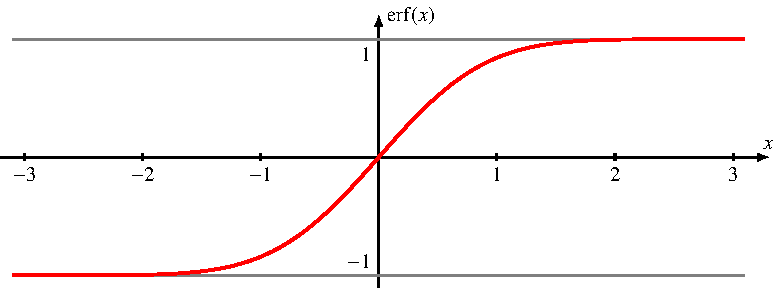
\includegraphics{chapters/060-integral/images/erf.pdf}
\caption{Graph der Fehlerunktion $\operatorname{erf}(x)$
\label{buch:integrale:fig:erf}}
\end{figure}
Die Funktion $\operatorname{erf}$ nimmt Werte zwischen $-1$ und $1$ an,
wie man in Abbildung~\ref{buch:integrale:fig:erf} sehen kann.
Die horizontalen Geraden $y=\pm 1$ sind Asymptoten.
Die exakte Berechnung von $\operatorname{erf}(x)$ für sehr grosse Werte
des Argumentes gestaltet sich schwierig, da es zur starker Auslöschung
kommen kann.
Da die Funktionswerte $\operatorname{erf}(x)$ sehr nahe bei $1$ sind,
lohnt es sich, nicht $\operatorname{erf}(x)$, sondern $1-\operatorname{erf}(x)$
zu berechnen.

\begin{definition}
\index{komplementäre Fehlerfunktion}
\index{Fehlerfunktion, komplementäre}
\index{erfc(x)@$\operatorname{erfc}(x)$}
Die {\em komplementäre Fehlerfunktion} ist die Funktion
\[
\operatorname{erfc}
\colon
\mathbb{R} \to [0,2]
:
x\mapsto
\operatorname{erfc}(x)
:=
1-\operatorname{erf}(x)
=
\frac{2}{\sqrt{\pi}}\int_x^\infty e^{-u^2}\,du.
\]
Die {\em verallgemeinerte Fehlerfunktion} ist definiert als
\[
\operatorname{erf}(a,b)
=
\frac{2}{\sqrt{\pi}}
\int_a^b e^{-u^2}\,du.
\]
\end{definition}

Mit der Fehlerfunktion kann die Standardnormalverteilungsfunktion jetzt
als
\[
\Phi(x)
=
\frac12
+
\frac12\operatorname{erf}\biggl( \frac{x}{\sqrt{2}} \biggr)
=
\frac12\biggl(
1+\operatorname{erf}\biggl(\frac{x}{\sqrt{2}}\biggr)\biggr)
\]
ausdrücken.
Die Verteilungsfunktion einer normalverteilten Zufallsvariable mit
Erwartungswert $\mu$ und Varianz $\sigma^2$ kann ebenfalls mit
\[
F_X(x)
=
\frac12\biggl(
1+\operatorname{erf}\biggl(\frac{x-\mu}{\sqrt{2}\sigma}\biggr)
\biggr)
\]
berechnet werden.
Die Fehlerfunktion ist also eine ``gute'' spezielle Funktion, die
die Berechnung von Wahrscheinlichkeitswerten von normalverteilten
Zufallsvariablen vereinfacht.

\subsection{Laplace-Transformation}
Wir berechnen die Laplace-Transformierte der Funktion
\[
f(t) = \operatorname{erf}\biggl(\frac{a}{2\sqrt{t}}\biggr).
\]
Nach Definition der Laplace-Transformation ist dies die Funktion
\begin{align*}
\mathscr{L}f(s)
&=
\int_0^\infty
e^{-st} \operatorname{erf}\biggl(\frac{a}{2\sqrt{t}}\biggr)
\,dt
=
\int_0^\infty
e^{-st}
\frac{2}{\sqrt{\pi}}
\int_0^{\frac{a}{2\sqrt{t}}}
e^{-x^2}
\,dx
\,dt.
\end{align*}
Das Integrationsgebiet $G$ ist der Teil des ersten Quadranten der
$t$-$x$-Ebene, für den die Ungleichung $x \le a/2\sqrt{t}$ gilt.
Dies ist gleichbedeutend mit $t \le a^2/4x^2$.
Vertauscht man die Integrationsreihenfolge, erhält man
\begin{align}
\mathscr{L}f(s)
&=
\int_G
e^{-st}
\frac{2}{\sqrt{\pi}}
e^{-x^2}
\,dx \,dt
=
\int_0^\infty
\int_0^{\frac{a^2}{4x^2}}
e^{-st}
\frac{2}{\sqrt{\pi}}
e^{-x^2}
\,dt
\,dx
=
\frac{2}{\sqrt{\pi}}
\int_0^\infty
e^{-x^2}
\int_0^{\frac{a^2}{4x^2}}
e^{-st}
\,dt
\,dx
\notag
\\
&=
\frac{2}{\sqrt{\pi}}
\int_0^\infty
e^{-x^2}
\biggl[
-\frac1{s}e^{-st}
\biggr]_0^{\frac{a^2}{4x^2}}
\,dx
=
\frac{2}{\sqrt{\pi}}
\int_0^\infty
e^{-x^2}
\frac1{s}
\biggl(
1-e^{-\frac{sa^2}{4x^2}}
\biggr)
\,dx
\notag
\\
&=
\frac{1}{s}
\cdot
\frac{2}{\sqrt{\pi}}\int_0^\infty e^{-x^2}\,dx
-
\frac1{s}
\cdot
\frac{2}{\sqrt{\pi}}
\int_0^\infty
e^{-x^2-\frac{sa^2}{4x^2}}
\,dx
\notag
\\
&=
\frac1s\lim_{x\to\infty} \operatorname{erf}(x)
-
\frac1s
\cdot
\frac{2}{\sqrt{\pi}}
\int_0^\infty e^{-\left(x^2+\frac{sa^2}{4x^2}\right)}\,dx.
\label{buch:integrale:eqn:laplaceerf}
\end{align}
Der Grenzwert im ersten Term ist nach Definition der Fehlerfunktion $1$. 
Schreiben wir $b=a\sqrt{s}/2$, dann wird das Integral im zweiten Term
\begin{equation}
I(b)
=
\int_0^\infty e^{-\left(x^2+\frac{sa^2}{4x^2}\right)}\,dx
=
\int_0^\infty \exp\biggl(-\biggl(x^2+\frac{b^2}{x^2}\biggr)\biggr)\,dx.
\label{buch:integrale:eqn:Ibsumme}
\end{equation}
Den Exponenten im Integranden kann man wie folgt als quadratischen
Ausdruck in $x\pm a/x$ schreiben:
\begin{equation*}
\begin{aligned}
%\biggl(
x^2 + \frac{b^2}{x^2}
%\biggr)
&=
\biggl(x+\frac{b}{x}\biggr)^2 - 2b
\\
&=
\biggl(x-\frac{b}{x}\biggr)^2 + 2b.
\end{aligned}
\end{equation*}
Man kann also das Integral $I(b)$ auf die eine oder andere Art als
\begin{equation}
\begin{aligned}
I(b)
&=
\int_0^\infty \exp\biggl(-\biggl(x+\frac{b}{x}\biggr)^2+2b\biggr)\,dx
\\
\text{oder}\quad\phantom{I(b)}
&=
\int_0^\infty \exp\biggl(-\biggl(x-\frac{b}{x}\biggr)^2-2b\biggr)\,dx
\end{aligned}
\label{buch:integrale:eqn:fehlerintegrale}
\end{equation}
schreiben.
Die Faktoren $e^{\pm 2b}$ können aus dem Integral genommen werden.
Trotzdem kann man das Integral nicht einfach ausführen.

Die Substitution $y=x\pm\frac{b}{x}$ vereinfacht den Integranden
\eqref{buch:integrale:eqn:fehlerintegrale}
zwar zu $e^{-y^2}$, aber die Substitution für $dx$ liefert
\begin{equation}
y=x\pm\frac{b}{x}
\qquad\Rightarrow\qquad
dy = \biggl(1\mp \frac{b}{x^2}\biggr)\,dx.
\label{buch:integrale:eqn:dy}
\end{equation}
Dies kann für die Berechnung von $I(b)$ verwendet werden.
Zunächst folgt aus \eqref{buch:integrale:eqn:fehlerintegrale},
dass jede konvexe Kombination der beiden Integrale mit Koeffizienten,
die sich zu $1$ summieren, wieder $I(b)$ erbibt.
Wählen wir die Koeffizienten 
\[
\frac12\biggl(1\mp\frac{b}{x^2}\biggr),
\]
dann heben sich die Terme mit $b/x^2$ weg, wir erhalten die
konvexe Kombination
\[
I(b)
=
\frac12
\cdot
\underbrace{
\int_0^\infty
\biggl(1-\frac{b}{x^2}\biggr)
\exp\biggl(-\biggl(x+\frac{b}{x}\biggr)^2\biggr)\,dx
}_{\displaystyle=I_+(b)}
\mathstrut
\cdot e^{2b}
+
\frac12
\underbrace{
\int_0^\infty
\biggl(1+\frac{b}{x^2}\biggr)
\exp\biggl(-\biggl(x-\frac{b}{x}\biggr)^2\biggr)\,dx
}_{\displaystyle=I_-(b)}
\mathstrut
\cdot e^{-2b},
\]
die aus zwei Integralen besteht, die einfacher berechnet werden können.

Im Integral $I_-(b)$ können wir die Substition \eqref{buch:integrale:eqn:dy}
und erhalten
\begin{align*}
I_-(b)
&=
\int_{-\infty}^\infty
\biggl(1+\frac{b}{x^2}\biggr)
\exp\biggl(-\biggl(x-\frac{b}{x}\biggr)^2\biggr)\,dx
=
\int_{-\infty}^\infty e^{-y^2}\,dy
=
\frac{\sqrt{\pi}}2
\end{align*}
nach Definition der Fehlerfunktion.

Das erste Integral $I_+(b)$ ist etwas schwieriger zu berechnen.
Die Substition $z=b/x$ bildet das Integrationsinterval auf sich selbst ab,
aber die Integrationsrichtung kehrt um.
Mit
\[
dz = -\frac{b}{x^2}\,dx
\qquad\Rightarrow\qquad
dx = -\frac{z^2}{b}\,dz
\]
erhalten wir jetzt
\begin{align*}
I_+(b)
&=
\int_0^\infty
\biggl(1-\frac{b}{x^2}\biggr)
\exp\biggl(-\biggl(x+\frac{b}{x}\biggr)^2\biggr)\,dx
\\
&=
\int_{\infty}^0
\biggl(1-\frac{b}{b^2/z^2}\biggr)
\exp\biggl(-\biggl(\frac{b}{z}+z\biggr)^2\biggr)\,
\biggl(-\frac{b}{z^2}\biggr)\,dz
\\
&=
\int_{0}^{\infty}
\biggl(1-\frac{b}{b^2/z^2}\biggr)
\exp\biggl(-\biggl(\frac{b}{z}+z\biggr)^2\biggr)\,
\frac{b}{z^2}\,dz
\\
&=
\int_{0}^{\infty}
\biggl(\frac{b}{z^2}-1\biggr)
\exp\biggl(-\biggl(\frac{b}{z}+z\biggr)^2\biggr)\,
dz
=
-I_+(b).
\end{align*}
Indem man auf beiden Seiten $I_+(b)$ addiert erhält man nun $2I_+(b)=0$,
also auch $I_+(b)=0$.
Das Integral $I_+(b)$ verschwindet also, $I_+(b)=0$.

Nach all diesen Zwischenrechnungen können wir jetzt das Integral $I(b)$
zusammensetzen.
Wir finden
\begin{align*}
I(b)
&=
\frac12e^{2b} I_+(b) +\frac12e^{-2b} I_-(b)
\\
&=
\frac12e^{-a\sqrt{s}}\cdot \frac{\sqrt{\pi}}{2}.
\end{align*}
Einsetzen in \eqref{buch:integrale:eqn:laplaceerf} gibt jetzt das
Resultat für die Laplace-Transformierte von $f(t)$, sie ist
\[
\mathscr{L}f(s)
=
\frac1s - \frac1s\cdot\frac{2}{\sqrt{\pi}} I(b)
=
\frac1s\biggl(1-\frac12e^{-a\sqrt{s}} \biggr).
\]

\begin{satz} Die Laplace-Transformierte der Fehlerfunktion mit Argument
$a/2\sqrt{t}$ ist
\begin{equation}
f(t) = \operatorname{erf}\biggl(\frac{a}{2\sqrt{t}}\biggr)
\qquad\multimapdotbothA\qquad
\mathscr{L}f(s)
=
\frac1s\biggl(1-\frac12e^{-a\sqrt{s}}\biggr).
\end{equation}
\end{satz}




\subsection{Berechnungsmethoden}
Die Fehlerfunktion kann natürlich mit numerischen Integrationsmethoden
berechnet werden.
Diese verlangen jedoch typischerweise die Auswertung des Integranden
an einer grossen Zahl von Stützstellen.
Im vorliegenden Falle müsste die transzendente Exponentialfunktion
sehr häufig berechnet werden, was zu sehr langer Laufzeit führt.
Gefragt sind daher Berechnungsverfahren, die möglichst nur arithmetische
Operationen verwenden, die sehr schnell in Hardware ausgeführt werden
können.

\subsubsection{Taylorreihe}
Die Fehlerfunktion ist das Integral einer Exponentialfunktion, die mit
Hilfe einer Potenzreihe für beliebige Argumente berechnet werden kann.
Aus
\[
e^x
=
1+x+\frac{x^2}{2!}+\frac{x^3}{3!} + \dots
=
\sum_{k=0}^\infty \frac{x^k}{k!}
\]
erhalten wir die Potenzreihe
\begin{equation}
e^{-t^2}
=
\sum_{k=0}^{\infty}
(-1)^k
\frac{t^{2k}}{k!},
\label{buch:integrale:eqn:erftaylor}
\end{equation}
die für alle Werte von $t$ konvergiert.

Da die Reihe
\eqref{buch:integrale:eqn:erftaylor}
absolut konvergiert, darf man sie gliedweise integrieren und erhält
\begin{equation}
\operatorname{erf}(x)
=
\frac{2}{\sqrt{\pi}}
\int_0^x
e^{-t^2}\,dt
=
\frac{2}{\sqrt{\pi}}
\sum_{k=0}^\infty \frac{(-1)^k}{k!}\int_0^x t^{2k}\,dt
=
\frac{2}{\sqrt{\pi}}
\sum_{k=0}^\infty \frac{(-1)^kx^{2k+1}}{k!(2k+1)}.
\label{buch:integrale:eqn:erfreihe}
\end{equation}
Diese Reihenentwicklung ist sehr effizient für kleine Werte von $x$.
Für grosse Werte von $x$ entstehen aber sehr grosse Zwischenterme in der
Reihe, was zu Auslöschung und damit zu Genauigkeitsverlust führt.

\subsubsection{Kettenbruchentwicklung}
Besonders für grosse $x$ interessiert man sich mehr für
$\operatorname{erfc}(x)$ als für $\operatorname{erf}(x)$.
Die Potenzreihe \eqref{buch:integrale:eqn:erfreihe} ist
dafür wegen der bereits erwähnten Auslöschung besonders ungeeignet.
Man kann aber die Kettenbruchentwicklung 
\begin{equation}
\operatorname{erfc}(z)
=
\frac{2ze^{-z^2}}{\sqrt{\pi}}
\cfrac{1}{
z+\cfrac{\frac12}{
z+\cfrac{\frac22}{
z+\cfrac{\frac32}{
z+\cfrac{\frac42}{
z+\cfrac{\frac52}{
z+\cfrac{\frac62}{
z+\dots}}}}}}}
\end{equation}
finden, die in \cite[p.~175]{buch:pade} dargestellt wird.
Für grosse $z$ liefert dieser Kettenbruch besonders schnell konvergierende
Näherungsbrüche für $\operatorname{erfc}(z)$.

\subsubsection{Interpolation}
Die GNU Scientific Library \cite{buch:library:gsl} verwendet eine Reihe von
Tschebyscheff-Approximationspolynomen, die für die Intervalle, in denen
sie definiert sind, besonders effizient zu berechnende Approximation
mit Maschinengenauigkeit ergeben.

%
% eulertransformation.tex
%
% (c) 2021 Prof Dr Andreas Müller, OST Ostschweizer Fachhochschule
%
\section{Euler-Transformation der hypergeometrischen Funktionen
\label{buch:integral:section:eulertransformation}}
\rhead{Euler-Transformation}
Die hypergeometrischen Funktionen wurden bisher einerseits
als Reihen mit einer speziellen Rekursionsrelation der Reihenglieder
und als Lösungen einer speziellen Art von Differentialgleichung
erkannt.
In diesem Abschnitt soll untersucht werden, ob man sie auch
auch durch Integrale definieren kann.

\subsection{Integraldarstellung der hypergeometrischen Funktion
$\mathstrut_2F_1$}

XXX An dieser Stelle Abschnitt 4.3.5 (Integraldarstellung) einfügen

\begin{satz}[Euler]
\label{buch:integrale:eulertransformation:satz}
Die hypergeometrische Funktion $\mathstrut_2F_1$ kann durch das 
Integral
\begin{equation}
\mathstrut_2F_1\biggl(\begin{matrix}a,b\\c\end{matrix};z\biggr)
=
\frac{\Gamma(c)}{\Gamma(b)\Gamma(c-b)}
\int_0^1
t^{b-1}(1-t)^{c-b-1}(1-zt)^{-a}
\,dt
\label{buch:integrale:eulertransformation:satzeqn}
\end{equation}
dargestellt werden.
\end{satz}

\subsubsection{Alternative Parametrisierungen}
Die Substitution $t=\sin^2 s$ ermöglicht eine alternative Parametrisierung
der Integraldarstellung der hypergeometrischen Funktion.
Wenden wir sie auf~\eqref{buch:integrale:eulertransformation:satzeqn}
an, erhalten wir wegen $dt = 2\cos s\sin s\,ds$
\begin{align*}
\mathstrut_2F_1\biggl(\begin{matrix}a,b\\c\end{matrix};z\biggr)
&=
\frac{\Gamma(c)}{\Gamma(b)\Gamma(c-b)}
\int_0^{\frac{\pi}2}
\sin^{2(b-1)}(s)\,
(1-\sin^2s)^{c-b-1} (1-z\sin^2 s)^{-a}
\,\cos s\sin s
\,ds
\\
&=
\frac{\Gamma(c)}{\Gamma(b)\Gamma(c-b)}
\int_0^{\frac{\pi}2}
\sin^{2b-1}(s)\,\cos^{2c-2b-1}(s)\, (1-z\sin^2 s)^{-a}
\,ds.
\end{align*}

XXX Parametrisierung für Intervall $[0,\infty)$

\subsection{Integraldarstellung als Integraltransformation}
Im vorangegangenen Abschnitt wurde gezeigt, wie sich die Funktion
$\mathstrut_2F_1$ als ein Integral des Integranden
\[
t^{b-1}(1-t)^{c-b-1} (1-xt)^{-a}
\]
ausdrücken lässt.
Der letzte Faktor $(1-xt)^{-a}$ kann mit der Binomialreihe
\begin{align*}
(1+x)^\alpha
&=
1
+ 
\alpha x
+
\frac{\alpha(\alpha-1)}{2!}x^2
+
\frac{\alpha(\alpha-1)(\alpha-2)}{3!}x^3
+
\\
&=
1
+
\frac{-\alpha}{1}(-x)
+
\frac{-\alpha(-\alpha+1)}{2!} (-x)^2
+
\frac{-\alpha(-\alpha+1)(-\alpha+2)}{3!} (-x)^3
+
\dots
\\
&=
\sum_{k=0}^\infty \frac{(-\alpha)_k}{k!} (-x)^k
=
\mathstrut_0F_1\biggl(
\begin{matrix}
\text{---}\\-\alpha
\end{matrix}
;-x
\biggr)
\end{align*}
als hypergeometrische Funktion geschrieben werden.
Die Integraldarstellung von $\mathstrut_2F_1$ kann daher auch als
\[
\mathstrut_2F_1\biggl(\begin{matrix}a,b\\c\end{matrix};z\biggr)
=
\frac{\Gamma(c)}{\Gamma(b)\Gamma(c-b)}
\int_0^1 t^{b-1}(1-t)^{c-b-1}
\,
\mathstrut_0F_1(;a;zt)\,dt
\]
Eine gewisse Ähnlichkeit zur Laplace-Transformation ist dieser
Formel nicht abzusprechen.
Die Funktion \( t^{b-1}(1-t)^{c-b-1} \) wird statt mit der
Exponentialfunktion $e^{xt} = \mathstrut_0F_0(xt)$ mit der
hypergeometrischen Funktion $\mathstrut_0F_1(;a;xt)$ multipliziert und
integriert.
Dies suggeriert, dass sich möglicherweise jede der hypergeometrischen
Funktionen $\mathstrut_{p+1}F_{q+1}$ durch ein Integral, dessen 
Integrand $\mathstrut pF_q$ enthält, ausdrücken lässt.

\begin{satz}
Es gilt
\[
\mathstrut_{p+1}F_{q+1}\biggl(
\begin{matrix}
a_1,\dots,a_{p+1}\\
b_1,\dots,b_{q+1}
\end{matrix}
;z
\biggr)
=
\frac{\Gamma(b_{q+1})}{\Gamma(a_{p+1})\Gamma(b_{q-1}-a_{p+1})}
\int_0^1
t^{a_{p+1}-1}(1-t)^{b_{q+1}-a_{p+1}-1}
\mathstrut_pF_q\biggl(
\begin{matrix}
a_1,\dots,a_p\\
b_1,\dots,b_q
\end{matrix};zt
\biggr)
\,dt
\]
\end{satz}

\begin{proof}[Beweis]
Sei $I$ das Integral auf der rechten Seite.
Wir setzen die Reihenentwicklung der Funktion $\mathstrut_pF_q$ in
die Integralformel ein und erhalten
\begin{align*}
I
&=
\int_0^1 t^{a_{p+1}-1}(1-t)^{b_{q+1}-a_{p+1}-1}
\sum_{k=0}^\infty
\frac{(a_1)_k\cdots (a_p)_k}{(b_1)_k\cdots (b_q)_k}
\frac{(zt)^k}{k!}
\,dt
\\
&=
\sum_{k=0}^\infty
\frac{(a_1)_k\cdots (a_p)_k}{(b_1)_k\cdots (b_q)_k}
\frac{z^k}{k!}
\int_0^1
t^{a_{p+1}+k-1}(1-t)^{b_{q+1}-a_{p+1}-1}
\,dt.
\intertext{Das verbleibende Integral auf der rechten Seite ist das
Beta-Integral $B(a_{p+1}+k, b_{q+1}-a_{p+1})$:
}
&=
\sum_{k=0}^\infty
\frac{(a_1)_k\cdots (a_p)_k}{(b_1)_k\cdots (b_q)_k}
\frac{z^k}{k!}
B(a_{p+1}+k, b_{q+1}-a_{p+1}).
\intertext{Mit der Rekursionsformel aus
Lemma~\ref{buch:rekursion:gamma:betareklemma}
für das Beta-Integral folgt}
&=
\sum_{k=0}^\infty
\frac{(a_1)_k\cdots (a_p)_k}{(b_1)_k\cdots (b_q)_k}
\frac{z^k}{k!}
\frac{(a_{p+1})_k}{(b_{q+1})_k} B(a_{p+1},b_{q+1}-a_{p+1})
\\
&=
\sum_{k=0}^\infty
\frac{(a_1)_k\cdots (a_{p+1})_k}{(b_1)_k\cdots (b_{q+})_k}
\frac{z^k}{k!}
\frac{\Gamma(a_{p+1})\Gamma(b_{q+1}-a_{p+1})}{\Gamma(b_{q+1})}
\\
&=
\frac{\Gamma(a_{p+1})\Gamma(b_{q+1}-a_{p+1})}{\Gamma(b_{q+1})}
\,\mathstrut_{p+1}F_{q+1}\biggl(
\begin{matrix}a_1,\dots,a_{p+1}\\
b_1,\dots,b_{q+1}
\end{matrix}; z\biggr).
\end{align*}
Auflösen nach $\mathstrut_{p+1}F_{q+1}$ ergibt die behauptete
Formel.
\end{proof}

Auch die Euler-Transformation lässt sich mit Hilfe der Substitution
$t=\sin^2 s$ in eine alternative Parametrisierung umschreiben.
Sie ist
\begin{align*}
\mathstrut_{p+1}F_{q+1}\biggl(
\begin{matrix}
a_1,\dots,a_{p+1}\\
b_1,\dots,b_{q+1}
\end{matrix}
;z
\biggr)
&=
\frac{2\Gamma(b_{q+1})}{\Gamma(a_{p+1})\Gamma(b_{q-1}-a_{p+1})}
\\
&\quad\times
\int_0^{\frac{\pi}2}
\sin^{2a_{p+1}-2}(s)\, \cos^{2b_{q+1}-2a_{p+1}-2}(s)
\,
\mathstrut_pF_q\biggl(
\begin{matrix}
a_1,\dots,a_p\\
b_1,\dots,b_q
\end{matrix};z\sin^2 s
\biggr)
\sin s\cos s
\,ds
\\
&=
\frac{2\Gamma(b_{q+1})}{\Gamma(a_{p+1})\Gamma(b_{q-1}-a_{p+1})}
\\
&\quad\times
\int_0^{\frac{\pi}2}
\sin^{2a_{p+1}-1}(s)\, \cos^{2b_{q+1}-2a_{p+1}-1}(s)
\,
\mathstrut_pF_q\biggl(
\begin{matrix}
a_1,\dots,a_p\\
b_1,\dots,b_q
\end{matrix};z\sin^2 s
\biggr)
\,ds.
\end{align*}

%
% differentialalgebren.tex
%
% (c) 2021 Prof Dr Andreas Müller, OST Ostschweizer Fachhochschule
%
\section{Differentialkörper und der Satz von Liouville
\label{buch:integrale:section:dkoerper}}
\rhead{Differentialkörper und der Satz von Liouville}
Das Problem der Darstellbarkeit eines Integrals in geschlossener
Form verlangt zunächst einmal nach einer Definition dessen, was man
als ``geschlossene Form'' akzeptieren will.
Die sogenannten {\em elementaren Funktionen} von
Abschnitt~\ref{buch:integrale:section:elementar}
bilden dafür den theoretischen Rahmen.
Das Problem ist dann die Frage zu beantworten, ob ein Integral eine
Stammfunktion hat, die eine elementare Funktion ist.
Der Satz von Liouville von Abschnitt~\ref{buch:integrale:section:liouville}
löst das Problem.

\subsection{Eine Analogie
\label{buch:integrale:section:analogie}}
% XXX Analogie: Formel für Polynom-Nullstellen 
% XXX           Stammfunktion als elementare Funktion
Das Analysis-Problem, eine Stammfunktion zu finden, ist analog zum
wohlbekannten algebraischen Problem, Nullstellen von Polynomen zu finden.
Wir entwickeln diese Analogie in etwas mehr Detail, um zu sehen, ob man
aus dem algebraischen Problem etwas über das Problem der Analysis
lernen kann.

Für ein Polynom $p(X) = a_nX^n+a_{n-1}X^{n-1}+\dots+a_1X+a_0\in\mathbb{C}[X]$
mit Koeffizienten $a_k\in\mathbb{C}$ ist es sehr einfach, für jede beliebige
komplexe Zahl $z\in\mathbb{C}$ den Wert $p(z)$ des Polynoms auszurechnen.
Ein paar wenige Rechenregeln genügen dazu, man kann leicht einem Kind 
beibringen, mit einem Taschenrechner so einen Wert auszurechnen.

Ähnlich sieht es mit der Ableitungsoperation aus. 
Einige wenige Ableitungsregeln, die man in der Analysis~I lernt,
erlauben, auf mehr oder weniger mechanische Art und Weise, jede
beliebige Funktion abzuleiten.
Man kann auch leicht einen Computer dazu programmieren, solche Ableitungen
symbolisch zu berechnen.

Aus dem Fundamentalsatz der Algebra, der von Gauss vollständig bewiesen
wurde, ist bekannt, dass jedes Polynom mit Koeffizienten in $\mathbb{C}$
genau so viele Lösungen in $\mathbb{C}$, wie der Grad des Polynoms angibt.
Dies ist aber ein Existenzsatz, er sagt nichts darüber aus, wie man diese
Lösungen finden kann.
In Spezialfällen, wie zum Beispiel für quadratische Polynome, gibt
es spezialsierte Lösungsverfahren, mit denen man Lösungen angeben kann.
Natürlich existieren numerische Methoden wie zum Beispiel das
Newton-Verfahren, mit dem man Nullstellen von Polynomen beliebig genau
bestimmen kann.

Der Fundamentalsatz der Integralrechnung besagt, dass jede stetige 
Funktion eine Stammfunktion hat, die bis auf eine Konstante eindeutig
bestimmt ist.
Auch dieser Existenzsatz gibt keinerlei Hinweise darauf, wie man die
Stammfunktion finden kann.
In der Analysis-Vorlesung lernt man viele Tricks, die in einer
beindruckenden Zahl von Spezialfällen ermöglichen, ein passende
Funktion anzugeben.
Man lernt auch numerische Verfahren kennen, mit denen sich Werte der
Stammfunktion, also bestimmte Integrale, mit beliebiger Genauigkeit
finden kann.

Die numerische Lösung des Nullstellenproblems ist insofern unbefriedigend,
als sie nur schwer eine Diskussion der Abhängigkeit der Nullstellen von
den Koeffizienten des Polynoms ermöglichen.
Eine Formel wie die Lösungsformel für die quadratische Gleichung 
stellt genau für solche Fälle ein ideales Werkzeug bereit.
Was man sich also wünscht ist nicht nur einfach eine Lösung, sondern eine
einfache Formel zur Bestimmung aller Lösungen.
Im Zusammenhang mit algebraischen Gleichungen erwartet man eine Formel,
in der nur arithmetische Operationen und Wurzeln vorkommen.
Für quadratische Gleichungen ist so eine Formel seit dem Altertum bekannt,
Formeln für die kubische Gleichung und die Gleichung vierten Grades wurden
im 16.~Jahrhundert von Cardano bzw.~Ferrari gefunden.
Erst viel später haben Abel und Ruffini gezeigt, dass so eine allgemeine
Formel für Polynome höheren Grades als 4 nicht existiert.
Die Galois-Theorie, die auf den Ideen von Évariste Galois beruht, 
stellt eine vollständige Theorie unter anderem für die Lösbarkeit
von Gleichungen durch Wurzelausdrücke dar.

Numerische Integralwerte haben ebenfalls den Nachteil, dass damit
Diskussionen wie die Abhängigkeit von Parametern eines Integranden
nur schwer möglich sind.
Was man sich daher wünscht ist eine Formel für die Stammfunktion,
die Werte als Zusammensetzung gut bekannter Funktionen wie der Exponential-
und Logarithmus-Funktionen oder der trigonometrischen Funktionen
sowie Wurzeln, Potenzen und den arithmetischen Operationen.
Man sagt, man möchte die Stammfunktion in ``geschlossener Form'' 
dargestellt haben.
Tatsächlich ist dieses Problem auch zu Beginn des 19.~Jahrhunderts
von Joseph Liouville genauer untersucht worden.
Er hat zunächst eine Klasse von ``elementaren Funktionen'' definiert,
die als Darstellungen einer Stammfunktion in Frage kommen.
Der Satz von Liouville besagt dann, dass nur Funktionen mit einer
ganz speziellen Form eine elementare Stammfunktion haben.
Damit wird es möglich, zu entscheiden, ob ein Integrand wie $e^{-x^2}$ 
eine elementare Stammfunktion hat.
Seit dieser Zeit weiss man zum Beispiel, dass die Fehlerfunktion nicht
mit den bekannten Funktionen dargestellt werden kann.

Mit dem Aufkommen der Computer und vor allem der Computer-Algebra-System (CAS)
wurde die Frage nach der Bestimmung einer Stammfunktion erneut aktuell.
Die ebenfalls weiter entwickelte abstrakte Algebra hat ermöglicht, die
Ideen von Liouville in eine erweiterte, sogenannte differentielle 
Galois-Theorie zu verpacken, die eine vollständige Lösung des Problems
darstellt.
Robert Henry Risch hat in den Sechzigerjahren auf dieser Basis
einen Algorithmus entwickelt, mit dem es möglich wird, zu entscheiden,
ob eine Funktion eine elementare Stammfunktion hat und diese
gegebenenfalls auch zu finden.
Moderne CAS implementieren diesen Algorithmus
in Teilen, besonders weit zu gehen scheint das quelloffene System
Axiom.

Der Risch-Algorithmus hat allerdings eine Achillesferse: er benötigt
eine Method zu entscheiden, ob zwei Ausdrücke übereinstimmen.
Dies ist jedoch ein im Allgemeinen nicht entscheidbares Problem.
Moderne CAS treiben einigen Aufwand, um die
Gleichheit von Ausdrücken zu entscheiden, sie können das Problem
aber grundsätzlich nicht vollständig lösen.
Damit kann der Risch-Algorithmus in praktischen Anwendungen das
Stammfunktionsproblem ebenfalls nur mit Einschränkungen lösen,
die durch die Fähigkeiten des Ausdrucksvergleichs in einem CAS
gesetzt werden.

Im Folgenden sollen elementare Funktionen definiert werden, es sollen
die Grundideen der differentiellen Galois-Theorie zusammengetragen werden
und der Satz von Liouvill vorgestellt werden.
An Hand der Fehler-Funktion soll dann gezeigt werden, wie man jetzt
einsehen kann, dass die Fehlerfunktion nicht elementar darstellbar ist.
Im nächsten Abschnitt dann soll der Risch-Algorithmus skizziert werden.

\subsection{Elementare Funktionen
\label{buch:integrale:section:elementar}}
Es soll die Frage beantwortet werden, welche Stammfunktionen sich
in ``geschlossener Form'' oder durch ``wohlbekannte Funktionen''
ausdrücken lassen.
Welche Funktionen dabei als ``wohlbekannt'' gelten dürfen ist
ziemlich willkürlich.
Sicher möchte man Potenzen und Wurzeln, Logarithmus und Exponentialfunktion,
aber auch die trigonometrischen Funktionen dazu zählen dürfen.
Ausserdem will man beliebig mit den arithmetischen Operationen
rechnen.
So entsteht die Menge der Funktionen, die man ``elementar'' nennen
will.

In der Menge der elementaren Funktionen möchte man jetzt
Stammfunktionen ausgewählter Funktionen suchen.
Dazu muss man von jeder Funktion ihre Ableitung kennen.
Die Ableitungsoperation macht aus der Funktionenmenge eine
differentielle Algebra.
Der Satz von Liouville (Satz~\ref{buch:integrale:satz:liouville1}) 
liefert Bedingungen, die erfüllt sein müssen, wenn eine Funktion
eine elementare Stammfunktion hat.
Sind diese Bedingungen nicht erfüllbar, ist auch keine 
elementare Stammfunktion möglich.

In den folgenden Abschnitten soll die differentielle Algebra
der elementaren Funktionen konstruiert werden.

\subsubsection{Körper}
Die einfachsten Funktionen sind die die Konstanten, für die wir
für die nachfolgenden Betrachtungen fast immer die komplexen Zahlen
$\mathbb{C}$
zu Grunde legen wollen.
Dabei ist vor allem wichtig, dass sich darin alle arithmetischen
Operationen durchführen lassen mit der einzigen Ausnahme, dass
nicht durch $0$ dividiert werden darf.
Man nennt $\mathbb{C}$ daher ein {\em Körper}.
\index{Körper}%
\label{buch:integrale:def:koerper}

\subsubsection{Polynome und rationale Funktionen}
Die Polynome einer Variablen beschreiben eine Menge von
Funktionen, in der Addition, Subtraktion, Multiplikation
von Funktionen und Multiplikation mit komplexen Zahlen
uneingeschränkt möglich ist.
Wir bezeichen wie früher die Menge der Polynome in $z$ mit
$\mathbb{C}[z]$.

Die Division ist erst möglich, wenn man beliebige Brüche
zulässt, deren Zähler und Nenner Polynome sind.
Die Menge
\[
\mathbb{C}(z)
=
\biggl\{
\frac{p(z)}{q(z)}
\;\bigg|\;
p,q\in \mathbb{C}[z]
\biggr\}
\]
heisst die Menge der {\em rationalen Funktionen}.
\label{buch:integrale:def:rationalefunktion}
\index{Funktion, rationale}%
\index{rationale Funktion}%
In ihr sind jetzt alle arithmetischen Operationen ausführbar
ausser natürlich die Division durch die Nullfunktion.
Die rationalen Funktionen bilden also wieder eine Körper.

Die Tatsache, dass die rationalen Funktionen einen Körper
bilden bedeutet auch, dass die Konstruktion erneut durchgeführt
werden kann.
Ausgehend von einem beliebigen Körper $K$ können wieder zunächst
die Polynome $K[X]$ und anschliesen die rationalen Funktionen $K[X]$
in der neuen Variablen, jetzt aber mit Koeffizienten in $K$
gebildet werden.
So entstehen Funktionen von mehreren Variablen und, indem
wir für die neue Variable $X$ zum Beispiel die im übernächsten
Abschnitt betrachtete Wurzel $X=\sqrt{z}$
einsetzen, rationale Funktionen in $z$ und $\sqrt{z}$.

Solche Funktionenkörper werden im folgenden mit geschweiften
Buchstaben $\mathscr{D}$ bezeichnet.
\index{Funktionenkörper}%

\subsubsection{Ableitungsoperation}
In allen Untersuchungen soll immer die Ableitungsoperation
mit berücksichtigt werden.
In unserer Betrachtungsweise spielt es keine Rolle, dass die
Ableitung aus einem Grenzwert entsteht, es sind nur die algebraischen
Eigenschaften wichtig.
Diese sind in der folgenden Definition zusammengefasst.

\begin{definition}
\label{buch:integrale:def:derivation}
Ein {\em Ableitungsoperator} oder eine {\em Derivation} einer Algebra
$\mathscr{D}$ von Funktionen ist eine lineare Abbildung
\[
\frac{d}{dz}
\colon \mathscr{D} \to \mathscr{D}
:
f \mapsto \frac{df}{dz} = f',
\]
die zusätzlich die Produktregel
\begin{equation}
\frac{d}{dz} (fg)
=
\frac{df}{dz} \cdot g + f \cdot \frac{dg}{dz}
\qquad\Leftrightarrow\qquad
(fg)' = f' g + fg'
\label{buch:integrale:eqn:produktregel}
\end{equation}
\index{Produktregel}%
erfüllt.
Die Funktion $f'\in \mathscr{D}$ heisst auch die {\em Ableitung}
von $f\in\mathscr{D}$.
\index{Derivation}%
\index{Ableitungsoperator}%
\index{Ableitung}%
\end{definition}

Die Produktregel hat zum Beispiel auch die bekannten Quotientenregel
zur Folge.
Dazu betrachten wir das Produkt $f= (f/g)\cdot g$ und leiten es mit
Hilfe der Produktregel ab:
\[
\frac{d}{dz}f
=
\frac{d}{dz}
\biggl(
\frac{f}{g}\cdot g
\biggr)
=
{\color{darkred}
\frac{d}{dz}
\biggl(
\frac{f}{g}
\biggr)}
\cdot g
+
\frac{f}{g}\cdot \frac{d}{dz}g.
\]
Jetzt lösen wir nach der {\color{darkred}roten} Ableitung des Quotienten
auf und erhalten
\begin{equation}
\biggl(\frac{f}{g}\biggr)'
=
\frac{d}{dz}\biggl(\frac{f}{g}\biggr)
=
\frac1g\biggl(
\frac{d}{dz}f - \frac{f}{g}\cdot \frac{d}{dz}g
\biggr)
=
\frac{1}{g}
\biggl(
f'-\frac{fg'}{g}
\biggr)
=
\frac{f'g-fg'}{g^2}.
\label{buch:integrale:eqn:quotientenregel}
\end{equation}
Dies ist die Quotientenregel.

Aus der Produktregel folgt natürlich sofort auch die Potenzregel
für die Ableitung der $n$ten Potenz einer Funktion $f\in\mathscr{D}$, 
sie lautet:
\begin{equation}
\frac{d}{dz} f^n
= 
\underbrace{
f'f^{n-1} + ff'f^{n-2} + f^2f'f^{n-3}+\dots f^{n-1}f'
}_{\displaystyle \text{$n$ Terme}}
=
nf^{n-1}f'.
\label{buch:integrale:eqn:potenzregel}
\end{equation}
In dieser Form versteckt sich natürlich auch die Kettenregel, die
Potenzfunktion ist die äussere Funktion, $f$ die innere, $f'$ ist also
die Ableitung er inneren Funktion, wie in der Kettenregel verlangt.
Falls $f$ ein Element von $\mathscr{D}$ ist mit der Eigenschaft
$df/dz=1$, dann entsteht die übliche Produktregel.

\begin{definition}
Eine Algebra $\mathscr{D}$ von Funktionen mit einem Ableitungsoperator 
$d/dz$ heisst eine {\em differentielle Algebra}.
\index{differentielle Algebra}%
\index{Algebra, differentielle}%
In einer differentiellen Algebra gelten die üblichen
Ableitungsregeln.
\end{definition}

Die Potenzregel war in der Form~\eqref{buch:integrale:eqn:potenzregel}
geschrieben worden, nicht als die Ableitung von $z$.
Der Grund dafür ist, dass wir gar nicht voraussetzen wollen, dass in
unserer differentiellen Algebra eine Funktion existiert, die die
Rolle von $z$ hat.
Dies ist gar nicht nötig, wie das folgende Beispiel zeigt.

\begin{beispiel}
Als Funktionenmenge $\mathscr{D}$ nehmen wir rationale Funktionen
in zwei Variablen, die wir $\cos x $ und $\sin x$ nennen.
Diese Menge bezeichnen wir mit
$\mathscr{D}=\mathbb{Q}(\cos x,\sin x)$
Der Ableitungsoperator ist 
\begin{align*}
\frac{d}{dx} \cos x &= -\sin x
\\
\frac{d}{dx} \sin x &= \phantom{-}\cos x.
\end{align*}
Die Funktionen von $\mathbb{Q}(\cos x,\sin x)$ sind also Brüche,
deren Zähler und Nenner Polynome in $\cos x$ und $\sin x$ sind.
Aus den Produkt- und Quotientenregeln und den Ableitungsregeln für
$\cos x$ und $\sin x$ folgt, dass die Ableitung einer Funktion in
$\mathscr{D}$ wieder in $\mathscr{D}$ ist, $\mathscr{D}$ ist eine
differentielle Algebra.
\end{beispiel}

Die konstanten Funktionen spielen eine besondere Rolle.
Da wir bei der Ableitung nicht von der Vorstellung einer
Funktion mit einem variablen Argument ausgehen wollten und 
die Ableitung nicht als Grenzwert definieren wollten, müssen
wir auch bei der Definition der ``Konstanten'' einen neuen
Weg gehen.
In der Analysis sind die Konstanten genau die Funktionen,
deren Ableitung $0$ ist.

\begin{definition}
\label{buch:integrale:def:konstante}
Ein Element $f\in \mathscr{D}$ mit $df/dz=f'=0$ heissen
{\em Konstante} in $\mathscr{D}$.
\index{Konstante}%
\end{definition}

Die in der Potenzregel~\eqref{buch:integrale:eqn:potenzregel}
vermisste Funktion $z$ kann man ähnlich zu den Konstanten
zu definieren versuchen.
$z$ müsste ein Element von $\mathscr{D}$ mit $z' = 1$ sein.
Allerdings gibt es viele solche Elemente, ist $c$ eine Konstanten
und $z'=1$, dann ist auch $(z+c)'=1$, $(z+c)$ hat also für
die Zwecke unserer Untersuchung die gleichen Eigenschaften wie
$z$.
Dies deckt sich natürlich auch mit der Erwartung, dass Stammfunktionen
nur bis auf eine Konstante bestimmt sind.
Eine differentielle Algebra muss allerdings kein Element $z$ mit der
Eigenschaft $z'=1$ enthalten.

\begin{beispiel}
In $\mathscr{D}=\mathbb{Q}(\cos x,\sin x)$ gibt es kein Element $x$.
Ein solches wäre von der Form
\[
x = \frac{p(\cos x,\sin x)}{q(\cos x,\sin x)}.
\]
Eine solche goniometrische Beziehung würde für $x=\frac{\pi}4$ bedeuten,
dass
\[
\frac{\pi}4
=
\frac{p(\sqrt{2}/2,\sqrt{2}/2)}{q(\sqrt{2}/2,\sqrt{2}/2)}.
\]
Auf der rechten Seite steht ein Quotient von Polynome, in dessen
Argument nur rationale Zahlen und $\sqrt{2}$ steht.
So ein Ausdruck kann immer in die Form
\[
\pi
=
4\frac{a\sqrt{2}+b}{c\sqrt{2}+d}
=
\frac{4(a\sqrt{2}+b)(c\sqrt{2}-d)}{2c^2+d^2}
=
r\sqrt{2}+s
\]
gebracht werden.
Die Zahl auf der rechten Seite ist zwar irrational, aber sie ist Nullstelle
des quadratischen Polynoms
\[
p(x)
=
(x-r\sqrt{2}-s)(x+r\sqrt{2}-s)
=
x^2
-2sx
-2r^2+s^2
\]
mit rationalen Koeffizienten, wie man mit der Lösungsformel für die
quadratische Gleichung nachprüfen kann.
Es ist bekannt, dass $\pi$ als transzendente Zahl nicht Nullstelle
eines Polynoms mit rationalen Koeffizienten ist.
Dieser Widerspruch zeigt, dass $x$ nicht in $\mathbb{Q}(\cos x, \sin x)$
vorkommen kann.
\end{beispiel}

In einer differentiellen Algebra kann jetzt die Frage nach der
Existenz einer Stammfunktion gestellt werden.

\begin{aufgabe}
\label{buch:integrale:aufgabe:existenz-stammfunktion}
Gegeben eine differentielle Algebra $\mathscr{D}$ und ein Element
$f\in\mathscr{D}$, entscheide, ob es ein Element $F\in\mathscr{D}$ 
gibt mit der Eigenschaft $F'=f$.
Ein solches $F\in\mathscr{D}$ heisst {\em Stammfunktion} von $f$.
\end{aufgabe}

\begin{satz}
In einer differentiellen Algebra $\mathscr{D}$ mit $z\in\mathscr{D}$
hat die Potenzfunktion $f=z^n$ für $n\in\mathbb{N}\setminus\{-1\}$
ein Stammfunktion, nämlich 
\[
F = \frac{1}{n+1} z^{n+1}.
\]
\label{buch:integrale:satz:potenzstammfunktion}
\end{satz}

\begin{proof}[Beweis]
Tatsächlich kann man dies sofort nachrechnen, muss allerdings die
Fälle $n+1 >0$ und $n+1<0$ unterscheiden, da die Potenzregel
\eqref{buch:integrale:eqn:potenzregel} nur für natürliche Exponenten
gilt.
Man erhält
\begin{align*}
n+1&>0\colon
&
\frac{d}{dz}\frac{1}{n+1}z^{n+1}
&=
\frac{1}{n+1}(n+1)z^{n+1-1}
=
z^n,
\\
n+1&<0\colon
&
\frac{d}{dz}\frac{1}{n+1}\frac{1}{z^{-(n+1)}}
&=
\frac{1}{n+1}\frac{1'z^{-(n+1)}-1(-(n+1))z^{-n-1-1}}{z^{-2n-2}}
\\
&&
&=
\frac{1}{n+1}
\frac{(n+1)z^n{-n-2}}{z^{-2n-2}}
\\
&&
&=
\frac{1}{z^{-n}}=z^n.
\end{align*}
Man beachte, dass in dieser Rechnung nichts anderes als die
algebraischen Eigenschaften der Produkt- und Quotientenregel
verwendet wurden.
\end{proof}

\subsubsection{Wurzeln}
Die Wurzelfunktionen sollen natürlich als elementare Funktionen
erlaubt sein.
Es ist bekannt, dass $\sqrt{z}\not\in \mathscr{D}=\mathbb{C}(z)$
ist, ein solches Element müsste also erst noch hinzugefügt werden.
Dabei muss auch seine Ableitung definiert werden.
Auch dabei dürfen wir nicht auf eine Grenzwertüberlegung zurückgreifen,
vielmehr müssen wir die Ableitung auf vollständig algebraische
Weise bestimmen.

Wir schreiben $f=\sqrt{z}$ und leiten die Gleichung $f^2=z$ nach $z$ ab.
Dabei ergibt sich nach der Potenzregel
\[
\frac{d}{dz}f^2 = 2f'f = \frac{d}{dz}z=1
\qquad\Rightarrow\qquad f' = \frac{1}{2f}.
\]
Diese Rechnung lässt sich auch auf $n$-Wurzeln $g=\root{n}\of{z}$ mit
der Gleichung $g^n = z$ verallgemeinern.
Die Ableitung der $n$-ten Wurzel ist
\begin{equation}
\frac{d}{dz}g^n
=
ng^{n-1} = \frac{d}{dz}z=1
\qquad\Rightarrow\qquad
\frac{d}{dz}g = \frac{1}{ng^{n-1}}.
\end{equation}
Es ist also möglich, eine differentielle Algebra $\mathscr{D}$ mit einer
$n$-ten Wurzel $g$ zu einer grösseren differentiellen Algebra $\mathscr{D}(g)$
zu erweitern, in der wieder alle Regeln für das Rechnen mit Ableitungen
erfüllt sind.

\subsubsection{Algebraische Elemente}
Die Charakterisierung der Wurzelfunktionen passt zwar zum verlangten
algebraischen Vorgehen, ist aber zu spezielle und nicht gut für die
nachfolgenden Untersuchengen geeignet.
Etwas allgemeiner ist der Begriff der algebraischen Elemente.

\begin{definition}
\label{buch:integrale:def:algebraisches-element}
Seien $K\subset L$ zwei Körper.
Ein Element $\alpha \in L$ heisst {\em algebraisch} über $K$,
wenn $\alpha$ Nullstelle eines Polynoms $p\in K[X]$ mit Koeffizienten
in $K$ ist.
\index{algebraisch}%
\end{definition}

Jedes Element $\alpha\in K$ ist algebraisch, da $\alpha$ Nullstelle
von $X-\alpha\in K[X]$ ist.
Die $n$tem Wurzeln eines Elemente $\alpha\in K$ sind ebenfalls algebraisch,
da sie Nullstellen des Polynoms $p(X) = X^n - \alpha$ sind.
Allerdings ist nicht klar, dass diese Wurzeln überhaupt existieren.
Nach dem Satz von Abel~\ref{buch:potenzen:satz:abel} gibt es aber
Nullstellen von Polynomen, die sich nicht als Wurzelausdrücke schreiben
lassen.
Der Begriff der algebraischen Elemente ist also allgemeiner als der
Begriff der Wurzel.

\begin{definition}
\label{buch:integrale:def:algebraisch-abgeschlossen}
Ein Körper $K$ heisst {\em algebraisch abgeschlossen}, wenn jedes Polynom mit
Koeffizienten in $K$ eine Nullstelle in $K$ hat.
\end{definition}

Der Körper $\mathbb{C}$ ist nach dem
Fundamentalsatz~\label{buch:potenzen:satz:fundamentalsatz}
der Algebra algebraisch abgeschlossen.
Da wir aber mit Funktionen arbeiten, müssen wir auch Wurzeln
von Funktionen finden können.
Dies ist nicht selbstverständlich, wie das folgende Beispiel zeigt.

\begin{beispiel}
Es gibt keine stetige Funktion $f\colon \mathbb{C}\to\mathbb{C}$, die
die Gleichung $f(z)^2 = z$ und $f(1)=1$ erfüllt.
Für die Argumente $z(t)= e^{it}$ folgt, dass $f(z(t)) = e^{it/2}$ sein
muss.
Setzt man aber $t=\pm \pi$ ein, ergeben sich die Werte
$f(z(\pm\pi))=e^{\pm i\pi/2}=\pm 1$, die beiden Grenzwerte
für $t\to\pm\pi$ sind also verschieden.
\end{beispiel}

Die Mathematik hat verschiedene ``Tricks'' entwickelt, wie mit diesem
Problem umgegangen werden kann: Funktionskeime, Garben, Riemannsche
Flächen.
Sie sind alle gleichermassen gut geeignet, das Problem zu lösen.
Für die vorliegende Aufgabe genügt es aber, dass es tatsächlich
immer ein wie auch immer geartetes Element gibt, welches Nullstelle
des Polynoms ist.

Ist $f$ eine Nullstelle des Polynoms $p(X)$ mit Koeffizienten in
$\mathscr{D}$, dann kann man die Ableitung wie folgt berechnen.
Zunächst leitet man $p(f)$ ab:
\begin{align}
0&=
\frac{d}{dz}(a_nf^n + a_{n-1}f^{n-1}+\ldots+a_1f+a_0)
\notag
\\
&=
a_n'f^n + a_{n-1}'f^{n-1}+\ldots+a_1'f+a_0'
+
na_nf^{n-1}f'
+
(n-1)a_nf^{n-2}f'
+
\ldots
+
a_2ff'
+
a_1f'
\notag
\\
&=
a_n'f^n + a_{n-1}'f^{n-1}+\ldots+a_1'f+a_0'
+
(
na_nf^{n-1}
+
(n-1)a_nf^{n-2}
+
\ldots
+
a_2f
+
a_1
)f'
\notag
\\
\Rightarrow
\qquad
f'&=\frac{
a_n'f^n + a_{n-1}'f^{n-1}+\dots+a_1'f+a_0'
}{
na_nf^{n-1}
+
(n-1)a_nf^{n-2}
+
\dots
+
a_1
}.
\label{buch:integrale:eqn:algabl}
\end{align}
Das einzige, was dabei schief gehen könnte ist, dass der Nenner ebenfalls
verschwindet.
Dieses Problem kann man dadurch lösen, dass man als Polynom das
sogenannte Minimalpolynom verwendet.

\begin{definition}
Das {\em Minimalpolynome} $m(X)$ eines algebraischen Elementes $\alpha$ ist
das Polynom kleinsten Grades, welches $m(\alpha)=0$ erfüllt.
\end{definition}

Da das Minimalpolynom den kleinstmöglichen Grad hat, kann der Nenner
von~\eqref{buch:integrale:eqn:algabl},
der noch kleineren Grad hat, unmöglich verschwinden.
Das Minimalpolynom ist auch im wesentlichen eindeutig.
Gäbe es nämlich zwei verschiedene Minimalpolynome $m_1$ und $m_2$,
dann müsste $\alpha$ auch eine Nullstelle des grössten gemeinsamen
Teilers $m_3=\operatorname{ggT}(m_1,m_2)$ sein.
Wären die beiden Polynome wesentlich verschieden, dann hätte $m_3$
kleineren Grad, im Widerspruch zur Definition des Minimalpolynoms.
Also unterscheiden sich die beiden Polynome $m_1$ und $m_2$ nur um
einen skalaren Faktor.

\subsubsection{Konjugation, Spur und Norm}
% Konjugation, Spur und Norm
Das Minimalpolynom eines algebraischen Elementes ist nicht
eindeutig bestimmt.
Zum Beispiel ist $\sqrt{2}$ algebraisch über $\mathbb{Q}$, das
Minimalpolynom ist $m(X)=X^2-2\in\mathbb{Q}[X]$. 
Es hat aber noch eine zweite Nullstelle $-\sqrt{2}$.
Mit rein algebraischen Mitteln sind die beiden Nullstellen $\pm\sqrt{2}$
nicht zu unterscheiden, erst die Verwendung der Vergleichsrelation
ermöglicht, sie zu unterscheiden.

Dasselbe gilt für die imaginäre Einheit $i$, die das Minimalpolynom
$m(X)=X^2+1\in\mathbb{R}[X]$ hat.
Hier gibt es nicht einmal mehr eine Vergleichsrelation, mit der man
die beiden Nullstellen unterscheiden könnte.
In der Tat ändert sich aus algebraischer Sicht nichts, wenn man in
allen Formeln $i$ durch $-i$ ersetzt.

Etwas komplizierter wird es bei $\root{3}\of{2}$.
Das Polynom $m=x^3-2\in\mathbb{Q}[X]$ hat $\root{3}\of{2}$ als
Nullstelle und dies ist auch tatsächlich das Minimalpolynom.
Das Polynom hat noch zwei weitere Nullstellen
\[
\alpha_+ = \frac{-1+i\sqrt{3}}{2}\root{3}\of{2}
\qquad\text{und}\qquad
\alpha_- = \frac{-1-i\sqrt{3}}{2}\root{3}\of{2}.
\]
Die beiden Lösungen gehen durch die Vertauschung von $i$ und $-i$ 
auseinander hervor.
Betrachtet man dasselbe Polynom aber als Polynom in $\mathbb{R}[X]$,
dann ist es nicht mehr das Minimalpolynom von $\root{3}\of{2}$, da
$X-\root{3}\of{2}\in\mathbb{R}[X]$ kleineren Grad und $\root{3}\of{2}$
als Nullstelle hat.
Indem man
\[
m(X)/(X-\root{3}\of{2})=X^2+\root{3}\of{2}X+\root{3}\of{2}^2=m_2(X)
\]
rechnet, bekommt man das Minimalpolynom der beiden Nullstellen $\alpha_+$
und $\alpha_-$.
Wir lernen aus diesen Beispielen, dass das Minimalpolynom vom Grundkörper
abhängig ist (Die Faktorisierung $(X-\root{3}\of{2})\cdot m_2(X)$ von
$m(X)$ ist in $\mathbb{Q}[X]$ nicht möglich) und dass wir keine 
algebraische Möglichkeit haben, die verschiedenen Nullstellen des
Minimalpolynoms zu unterscheiden.

Die beiden Nullstellen $\alpha_+$ und $\alpha_-$ des Polynoms $m_2(X)$
erlauben, $m_2(X)=(X-\alpha_+)(X-\alpha_-)$ zu faktorisieren.
Durch Ausmultiplizieren
\[
(X-\alpha_+)(X-\alpha_-)
=
X^2 -(\alpha_++\alpha_-)X+\alpha_+\alpha_-
\]
und Koeffizientenvergleich mit $m_2(X)$ findet man die symmetrischen 
Formeln
\[
\alpha_+ + \alpha_- = \root{3}\of{2}
\qquad\text{und}\qquad
\alpha_+ \alpha_ = \root{3}\of{2}.
\]
Diese Ausdrücke sind nicht mehr abhängig von einer speziellen Wahl
der Nullstellen.

Das Problem verschärft sich nocheinmal, wenn wir Funktionen betrachten.
Das Polynom $m(X)=X^3-z$ ist das Minimalpolynom der Funktion $\root{3}\of{z}$.
Die komplexe Zahl $z=re^{i\varphi}$ hat aber drei die algebraisch nicht
unterscheidbaren Nullstellen 
\[
\alpha_0(z)=\root{3}\of{r}e^{i\varphi/3},
\quad
\alpha_1(z)=\root{3}\of{r}e^{i\varphi/3+2\pi/3}
\qquad\text{und}\qquad
\alpha_2(z)=\root{3}\of{r}e^{i\varphi/3+4\pi/3}.
\]
Aus der Faktorisierung $ (X-\alpha_0(z)) (X-\alpha_1(z)) (X-\alpha_2(z))$
und dem Koeffizientenvergleich mit dem Minimalpolynom kann man wieder
schliessen, dass die Relationen
\[
\alpha_0(z) + \alpha_1(z) + \alpha_2(z)=0
\qquad\text{und}\qquad
\alpha_0(z)  \alpha_1(z) \alpha_2(z) = z
\]
gelten.

Wir können also oft keine Aussagen über individuelle Nullstellen
eines Minimalpolynoms machen, sondern nur über deren Summe oder
Produkt.

\begin{definition}
\index{buch:integrale:def:spur-und-norm}
Sie $m(X)\in K[X]$ das Minimalpolynom eines über $K$ algebraischen
Elements und
\[
m(X) = a_nX^n + a_{n-1}X^{n-1} + \ldots + a_1X + a_0.
\]
Dann heissen
\[
\operatorname{Tr}(\alpha) = -a_{n-1}
\qquad\text{und}\qquad
\operatorname{Norm}(\alpha) = (-1)^n a_0
\]
die {\em Spur} und die {\em Norm} des Elementes $\alpha$.
\index{Spur eines algebraischen Elementes}%
\index{Norm eines algebraischen Elementes}%
\end{definition}

Die Spur und die Norm können als Spur und Determinante einer Matrix
verstanden werden, diese allgemeineren Definitionen, die man in der
Fachliteratur, z.~B.~in~\cite{buch:lang} nachlesen kann, führen aber
für unsere Zwecke zu weit.

\begin{hilfssatz}
Die Ableitungen von Spur und Norm sind
\[
\operatorname{Tr}(\alpha)'
=
\operatorname{Tr}(\alpha')
\qquad\text{und}\qquad
\operatorname{Norm}(\alpha)'
=
\operatorname{Tr}(\alpha)'
\]
XXX Wirklich?
\end{hilfssatz}

\subsubsection{Logarithmen und Exponentialfunktionen}
Die Funktion $z^{-1}$ musste im
Satz~\ref{buch:integrale:satz:potenzstammfunktion}
ausgeschlossen werden, sie hat keine Stammfunktion in $\mathbb{C}(z)$.
Aus der Analysis ist bekannt, dass die Logarithmusfunktion $\log z$ 
eine Stammfunktion ist.
Der Logarithmus von $z$ aber auch der Logarithmus $\log f(z)$
einer beliebigen Funktion $f(z)$ oder die Exponentialfunktion $e^{f(z)}$
sollen ebenfalls elementare Funktionen sein.
Da wir aber auch hier nicht auf die analytischen Eigenschaften zurückgreifen
wollen, brauchen wir ein rein algebraische Definition.

\begin{definition}
\label{buch:integrale:def:logexp}
Sei $\mathscr{D}$ ein differentielle Algebra und $f\in\mathscr{D}$.
Ein Element $\vartheta\in\mathscr{D}$ heisst ein {\em Logarithmus}
von $f$, geschrieben $\vartheta = \log f$, wenn $f\vartheta' = f'$ gilt.
$\vartheta$ heisst eine Exponentialfunktion von $f$ wenn
$\vartheta'=\vartheta f'$ gilt.
\end{definition}

Die Formel für die Exponentialfunktion ist etwas vertrauter, sie ist
die bekannte Kettenregel
\begin{equation}
\vartheta'
=
\frac{d}{dz} e^f
=
e^f \cdot \frac{d}{dz} f
=
\vartheta \cdot f'.
\label{buch:integrale:eqn:exponentialableitung}
\end{equation}
Da wir uns vorstellen, dass Logarithmen Umkehrfunktionen von 
Exponentialfunktionen sein sollen, 
muss die definierende Gleichung genau wie
\eqref{buch:integrale:eqn:exponentialableitung}
aussehen, allerdings mit vertauschten Plätzen von $f$ und $\vartheta$,
also 
\begin{equation}
\vartheta' = \vartheta\cdot f'
\qquad
\rightarrow
\qquad
f' = f\cdot \vartheta'
\;\Leftrightarrow\;
\vartheta' = (\log f)' = \frac{f'}{f}.
\label{buch:integrale:eqn:logarithmischeableitung}
\end{equation}
Dies ist die aus der Analysis bekannte Formel für die logarithmische
Ableitung.

Der Logarithmus von $f$ und die Exponentialfunktion von $f$ sollen
also ebenfalls als elementare Funktionen betrachtet werden.

\subsubsection{Die trigonometrischen Funktionen}
Die bekannten trigonometrischen Funktionen und ihre Umkehrfunktionen
sollten natürlich auch elementare Funktionen sein.
Dabei kommt uns zur Hilfe, dass sie sich mit Hilfe der Exponentialfunktion
als
\[
\cos f = \frac{e^{if}+e^{-if}}2
\qquad\text{und}\qquad
\sin f = \frac{e^{if}-e^{-if}}{2i}
\]
schreiben lassen.
Eine differentielle Algebra, die die Exponentialfunktionen von $if$ und
$-if$ enthält, enthält also automatisch auch die trigonometrischen
Funktionen.
Im Folgenden ist es daher nicht mehr nötig, die trigonometrischen
Funktionen speziell zu untersuchen.

\subsubsection{Elementare Funktionen}
Damit sind wir nun in der Lage, den Begriff der elementaren Funktion
genau zu fassen.

\begin{definition}
\label{buch:integrale:def:einfache-elementare-funktion}
Sie $\mathscr{D}$ eine differentielle Algebra über $\mathbb{C}$ und
$\mathscr{D}(\vartheta)$ eine Erweiterung von $\mathscr{D}$ um eine
neue Funktion $\vartheta$, dann heissen $\vartheta$ und die Elemente
von $\mathscr{D}(\vartheta)$ einfach elementar, wenn eine der folgenden
Bedingungen erfüllt ist:
\begin{enumerate}
\item $\vartheta$ ist algebraisch über $\mathscr{D}$, d.~h.~$\vartheta$
ist eine ``Wurzel''.
\item $\vartheta$ ist ein Logarithmus einer Funktion in $\mathscr{D}$,
d.~h.~es gibt $f\in \mathscr{D}$ mit $f'=f\vartheta'$
(Definition~\ref{buch:integrale:def:logexp}).
\item $\vartheta$ ist eine Exponentialfunktion einer Funktion in $\mathscr{D}$,
d.~h.~es bit $f\in\mathscr{D}$ mit $\vartheta'=\vartheta f'$
(Definition~\ref{buch:integrale:def:logexp}).
\end{enumerate}
\end{definition}

Einfache elementare Funktionen entstehen also ausgehend von einer 
differentiellen Algebra, indem man genau einmal eine Wurzel, einen
Logarithmus oder eine Exponentialfunktion hinzufügt.
So etwas wie die zusammengesetzte Funktion $e^{\sqrt{z}}$ ist
damit noch nicht möglich.
Daher erlauben wir, dass man die gesuchten Funktionen in mehreren
Schritten aufbauen kann.

\begin{definition}
Sei $\mathscr{F}$ eine differentielle Algebra, die die differentielle
Algebra $\mathscr{D}$ enthält, also $\mathscr{D}\subset\mathscr{F}$.
$\mathscr{F}$ und die Elemente von $\mathscr{F}$ heissen einfach,
wenn es endlich viele Elemente $\vartheta_1,\dots,\vartheta_n$ gibt
derart, dass
\[
\renewcommand{\arraycolsep}{2pt}
\begin{array}{ccccccccccccc}
\mathscr{D}
&\subset&
\mathscr{D}(\vartheta_1)
&\subset&
\mathscr{D}(\vartheta_1,\vartheta_2)
&\subset&
\;
\cdots
\;
&\subset&
\mathscr{D}(\vartheta_1,\vartheta_2,\dots,\vartheta_{n-1})
&\subset&
\mathscr{D}(\vartheta_1,\vartheta_2,\dots,\vartheta_{n-1},\vartheta_n)
&=&
\mathscr{F}
\\
\|
&&
\|
&&
\|
&&
&&
\|
&&
\|
&&
\\
\mathscr{F}_0
&\subset&
\mathscr{F}_1
&\subset&
\mathscr{F}_2
&\subset&
\cdots
&\subset&
\mathscr{F}_{n-1}
&\subset&
\mathscr{F}_{n\mathstrut}
&&
\end{array}
\]
gilt so, dass jedes $\vartheta_{i+1}$ einfach ist über 
$\mathscr{F}_i=\mathscr{D}(\vartheta_1,\dots,\vartheta_i)$.
\end{definition}

In Worten bedeutet dies, dass man den Funktionen von $\mathscr{D}$ 
nacheinander Wurzeln, Logarithmen oder Exponentialfunktionen einzelner
Funktionen hinzufügt.
Die Aufgabe~\ref{buch:integrale:aufgabe:existenz-stammfunktion} kann
jetzt so formuliert werden.

\begin{aufgabe}
\label{buch:integrale:aufgabe:existenz-stammfunktion-dalg}
Gegeben ist eine Differentielle Algebra $\mathscr{D}$ und eine
Funktion $f\in \mathscr{D}$.
Gibt es eine Folge $\vartheta_1,\dots,\vartheta_n$ und eine Funktion
$F\in\mathscr{D}(\vartheta_1,\dots,\vartheta_n)$ derart, dass
$F'=f$.
\end{aufgabe}

Das folgende Beispiel zeigt, wie man möglicherweise mehrere 
Erweiterungsschritte vornehmen muss, um zu einer Stammfunktion
zu kommen.
Es illustriert auch die zentrale Rolle, die der Partialbruchzerlegung
in der weiteren Entwicklung zukommen wird.

\begin{beispiel}
\label{buch:integrale:beispiel:nichteinfacheelementarefunktion}
Es soll eine Stammfunktion der Funktion
\[
f(z)
=
\frac{z}{(az+b)(cz+d)}
\in
\mathbb{C}(z)
\]
gefunden werden.
In der Analysis lernt man, dass solche Integrale mit der
Partialbruchzerlegung 
\[
\frac{z}{(az+b)(cz+d)}
=
\frac{A_1}{az+b}+\frac{A_2}{cz+d}
=
\frac{A_1cz+A_1d+A_2az+A_2b}{(az+b)(cz+d)}
\quad\Rightarrow\quad
\left\{
\renewcommand{\arraycolsep}{2pt}
\begin{array}{rcrcr}
cA_1&+&aA_2&=&1\\
dA_1&+&bA_2&=&0
\end{array}
\right.
\]
bestimmt werden.
Die Lösung des Gleichungssystems ergibt
$A_1=b/(bc-ad)$ und $A_2=d/(ad-bc)$.
Die Stammfunktion kann dann aus
\begin{align*}
\int f(z)\,dz
&=
\int\frac{A_1}{az+b}\,dz
+
\int\frac{A_2}{cz+d}\,dz
=
\frac{A_1}{a}\int\frac{a}{az+b}\,dz
+
\frac{A_2}{c}\int\frac{c}{cz+d}\,dz
\end{align*}
bestimmt werden.
In den Integralen auf der rechten Seite ist der Zähler jeweils die
Ableitung des Nenners, der Integrand hat also die Form $g'/g$.
Genau diese Form tritt in der Definition eines Logarithmus auf.
Die Stammfunktion ist jetzt
\[
F(z)
=
\int f(z)\,dz
=
\frac{A_1}{a}\log(az+b)
+
\frac{A_2}{c}\log(cz+d)
=
\frac{b\log(az+b)}{a(bc-ad)}
+
\frac{d\log(cz+d)}{c(ad-bc)}.
\]
Die beiden Logarithmen kann man nicht durch rein rationale Operationen
ineinander überführen.
Sie müssen daher beide der Algebra $\mathscr{D}$ hinzugefügt werden.
\[
\left.
\begin{aligned}
\vartheta_1&=\log(az+b)\\
\vartheta_2&=\log(cz+d)
\end{aligned}
\quad
\right\}
\qquad\Rightarrow\qquad
F(z) \in \mathscr{F}=\mathscr{D}(\vartheta_1,\vartheta_2).
\]
Die Stammfunktion $F(z)$ ist also keine einfache elementare Funktion,
aber $F$ ist immer noch eine elementare Funktion.
\end{beispiel}

\subsection{Partialbruchzerlegung
\label{buch:integrale:section:partialbruchzerlegung}}
Die Konstruktionen des letzten Abschnitts haben gezeigt,
wie man die Funktionen, die man als Stammfunktionen einer Funktion
zulassen möchte, schrittweise konstruieren kann.
Die Aufgabe~\ref{buch:integrale:aufgabe:existenz-stammfunktion-dalg}
ist eine rein algebraische Formulierung der ursprünglichen
Aufgabe~\ref{buch:integrale:aufgabe:existenz-stammfunktion}.
Schliesslich hat das Beispiel auf
Seite~\pageref{buch:integrale:beispiel:nichteinfacheelementarefunktion}
gezeigt, dass es im allgemeinen mehrere Schritte braucht, um zu einer
elementaren Stammfunktion zu gelangen.
Die Lösung setzt sich aus den Termen der Partialbruchzerlegung.
In diesem Abschnitt soll diese genauer studiert werden.

In diesem Abschnitt gehen wir immer von einer differentiellen
Algebra über den komplexen Zahlen aus und verlangen, dass die
Konstanten in allen betrachteten differentiellen Algebren
$\mathbb{C}$ sind.

\subsubsection{Monome}
Die beiden Funktionen $\vartheta-1=\log(az+b)$ und $\vartheta_2=(cz+d)$,
die im Beispiel hinzugefügt werden mussten, verhalten sich ich algebraischer
Hinsicht wie ein Monom: man kann es nicht faktorisieren oder bereits
bekannte Summanden aufspalten.
Solchen Funktionen kommt eine besondere Bedeutung zu.

\begin{definition}
\label{buch:integrale:def:monom}
Die Funktion $\vartheta$ heisst ein Monom, wenn $\vartheta$ nicht
algebraisch ist über $\mathscr{D}$ und $\mathscr{D}(\vartheta)$ die
gleichen Konstanten enthält wie $\mathscr{D}$.
\end{definition}

\begin{beispiel}
Als Beispiel beginnen wir mit den komplexen Zahlen $\mathbb{C}$
und fügen die Funktion $\vartheta_1=z$ hinzu und erhalten
$\mathscr{D}=\mathbb{C}(z)$.
Die Funktionen $z^k$ sind für alle $k$ linear unabhängig, d.~h.~es
gibt keinen Ausdruck
\[
a_nz^n + a_{n-1}z^{n-1}+\cdots+a_1z+a_0=0.
\]
Dies ist gleichbedeutend damit, dass $z$ nicht algebraisch ist.
Das Monom $z$ ist also auch ein Monom im Sinne der
Definition~\ref{buch:integrale:def:monom}.
\end{beispiel}

\begin{beispiel}
Wir beginnen wieder mit $\mathbb{C}$ und fügen die Funktion
$e^z$ hinzu.
Gäbe es eine Beziehung
\[
b_m(e^z)^m + b_{m-1}(e^z)^{m-1}+\dots+b_1e^z + b_0=0
\]
mit komplexen Koeffizienten $b_i\in\mathbb{C}$,
dann würde daraus durch Einsetzen von $z=1$ die Relation
\[
b_me^m + b_{m-1}e^{m-1} + \dots + b_1e + b_0=0,
\]
die zeigen würde, dass $e$ eine algebraische Zahl ist.
Es ist aber bekannt, dass $e$ transzendent ist.
Dieser Widersprich zeigt, dass $e^z$ ein Monom ist.
\end{beispiel}

\begin{beispiel}
Jetzt fügen wir die Exponentialfunktion $\vartheta_2=e^z$
der differentiellen Algebra $\mathscr{D}=\mathbb{C}(z)$ hinzu
und erhalten $\mathscr{F}_1=\mathscr{D}(e^z) = \mathbb{C}(z,e^z)$.
Gäbe es das Minimalpolynom 
\begin{equation}
b_m(z)(e^z)^m + b_{m-1}(z)(e^z)^{m-1}+\dots+b_1(z)e^z + b_0(z)=0
\label{buch:integrale:beweis:exp-analytisch}
\end{equation}
mit Koeffizienten $b_i\in\mathbb{C}(z)$, dann könnte man mit dem
gemeinsamen Nenner der Koeffizienten durchmultiplizieren und erhielte
eine Relation~\eqref{buch:integrale:beweis:exp-analytisch} mit
Koeffizienten in $\mathbb{C}[z]$.
Dividiert man durch $e^{mz}$ erhält man
\[
b_m(z) + b_{m-1}(z)\frac{1}{e^z} + \dots + b_1(z)\frac{1}{(e^z)^{m-1}} + b_0(z)\frac{1}{(e^z)^m}=0.
\]
Aus der Analysis weiss man, dass die Exponentialfunktion schneller
anwächst als jedes Polynom, alle Terme auf der rechten Seite
konvergieren daher gegen 0 für $z\to\infty$.
Das bedeutet, dass $b_m(z)\to0$ für $z\to \infty$.
Das Polynom~\eqref{buch:integrale:beweis:exp-analytisch} wäre also gar
nicht das Minimalpolynom.
Dieser Widerspruch zeigt, dass $e^z$ nicht algebraisch ist über
$\mathbb{C}(z)$ und damit ein Monom ist\footnote{Etwas unbefriedigend
an diesem Argument ist, dass man hier wieder rein analytische statt
algebraische Eigenschaften von $e^z$ verwendet.
Gäbe es aber eine minimale Relation wie
\eqref{buch:integrale:beweis:exp-analytisch}
mit Polynomkoeffizienten, dann wäre sie von der Form
\[
P(z,e^z)=p(z)(e^z)^m + q(z,e^z)=0,
\]
wobei Grad von $e^z$ in $q$ höchstens $m-1$ ist.
Die Ableitung wäre dann
\[
Q(z,e^z)
=
mp(z)(e^z)^m + p'(z)(e^z)^m + r(z,e^z)
=
(mp(z) + p'(z))(e^z)^m + r(z,e^z)
=0,
\]
wobei der Grad von $e^z$ in $r$ wieder höchstens $m-1$ ist.
Bildet man $mP(z,e^z) - Q(z,e^z) = 0$ ensteht eine Relation,
in der der Grad des Koeffizienten von $(e^z)^m$ um eins abgenommen hat.
Wiederholt man dies $m$ mal, verschwindet der Term $(e^z)^m$, die
Relation~\eqref{buch:integrale:beweis:exp-analytisch}
war also gar nicht minimal.
Dieser Widerspruch zeigt wieder, dass $e^z$ nicht algebraisch ist,
verwendet aber nur die algebraischen Eigenschaften der differentiellen
Algebra.
}.
\end{beispiel}

\begin{beispiel}
Wir hätten auch in $\mathbb{Q}$ arbeiten können und $\mathbb{Q}$
erst die Exponentialfunktion $e^z$ und dann den Logarithmus $z$ von $e^z$
hinzufügen können.
Es gibt aber noch weitere Logarithmen von $e^z$ zum Beispiel $z+2\pi i$.
Offenbar ist $\psi=z+2\pi i\not\in \mathbb{Q}(z,e^z)$, wir könnten also
auch noch $\psi$ hinzufügen.
Zwar ist $\psi$ auch nicht algebraisch, aber wenn wir $\psi$ hinzufügen,
dann wird aber die Menge der Konstanten grösser, sie umfasst jetzt
$\mathbb{Q}(2\pi i)$.
Die Bedingung in der Definition~\ref{buch:integrale:def:monom},
dass die Menge der Konstanten nicht grösser werden darf, ist also
verletzt.

Hätte man mit $\mathbb{Q}(e^z, z+2\pi i)$ begonnen, wäre $z$ aus
dem gleichen Grund kein Monom, aber $z+2\pi i$ wäre eines im Sinne
der Definition~\ref{buch:integrale:def:monom}.
In allen Rechnungen könnte man $\psi=z+2\pi i$ nicht weiter aufteilen,
da $\pi$ oder seine Potenzen keine Elemente von $\mathbb{Q}(e^z)$ sind.
\end{beispiel}

Da wir im Folgenden davon ausgehen, dass die Konstanten unserer
differentiellen Körper immer $\mathbb{C}$ sind, wird es jeweils
genügen zu untersuchen, ob eine neu hinzuzufügende Funktion algebraisch
ist oder nicht.

\subsubsection{Ableitungen von Polynomen und rationalen Funktionen von Monomen}
Fügt man einer differentiellen Algebra ein Monom hinzu, dann lässt
sich etwas mehr über Ableitungen von Polynomen oder Brüchen in diesen
Monomen sagen.
Diese Eigenschaften werden später bei der Auflösung der Partialbruchzerlegung
nützlich sein.

\begin{satz}
\label{buch:integrale:satz:polynom-ableitung-grad}
Sei
\[
P
=
A_nX^n + A_{n-1}X^{n-1} + \dots A_1X+A_0
\in\mathscr{D}[X]
\]
ein Polynom mit Koeffizienten in einer differentiellen Algebra $\mathscr{D}$
und $\vartheta$ ein Monom über $\mathscr{D}$.
Dann gilt
\begin{enumerate}
\item
\label{buch:integrale:satz:polynom-ableitung-grad-log}
Falls $\vartheta=\log f$ ist, ist $P(\vartheta)'$ ein
Polynom vom Grad $n$ in $\vartheta$, wenn der Leitkoeffizient $A_n$
nicht konstant ist, andernfalls ein Polynom vom Grad $n-1$.
\item
\label{buch:integrale:satz:polynom-ableitung-grad-exp}
Falls $\vartheta = \exp f$ ist, dann ist $P(\vartheta)'$ ein Polynom
in $\vartheta$ vom Grad $n$.
\end{enumerate}
\end{satz}

Der Satz macht also genaue Aussagen darüber, wie sich der Grad eines
Polynoms in $\vartheta$ beim Ableiten ändert.

\begin{proof}[Beweis]
Für Exponentialfunktion ist $\vartheta'=\vartheta f'$, die Ableitung
fügt also einfach einen Faktor $f'$ hinzu.
Terme der Form $A_k\vartheta^k$ haben die Ableitung
\[
(A_k\vartheta^k)
=
A'_k\vartheta^k + A_kk\vartheta^{k-1}\vartheta'
=
A'_k\vartheta^k + A_kk\vartheta^{k-1}\vartheta f'
=
(A'_k + kA_k f)\vartheta^k.
\]
Damit wird die Ableitung des Polynoms
\begin{equation}
P(\vartheta)'
=
\underbrace{(A'_n+nA_nf')\vartheta^n}_{\displaystyle=(A_n\vartheta^n)'}
+
(A'_{n-1}+(n-1)A_{n-1}f')\vartheta^{n-1}
+ \dots + 
(A'_1+A_1f')\vartheta + A_0'.
\label{buch:integrale:ableitung:polynom}
\end{equation}
Der Grad der Ableitung kann sich also nur ändern, wenn $A_n'+nA_nf'=0$ ist.
Dies bedeutet aber wegen
\(
(A_n\vartheta^n)'
=
0
\), dass  $A_n\vartheta^n=c$ eine Konstante ist.
Da alle Konstanten bereits in $\mathscr{D}$ sind, folgt, dass
\[
\vartheta^n=\frac{c}{A_n}
\qquad\Rightarrow\qquad
\vartheta^n - \frac{c}{A_n}=0,
\]
also wäre $\vartheta$ algebraisch über $\mathscr{D}$, also auch kein Monom.
Dieser Widerspruch zeigt, dass der Leitkoeffizient nicht verschwinden kann.

Für die erste Aussage ist die Ableitung der einzelnen Terme des Polynoms
\[
(A_k\vartheta^k)'
=
A_k'\vartheta^k + A_kk\vartheta^{k-1}\vartheta'
=
A_k'\vartheta^k + A_kk\vartheta^{k-1}\frac{f'}{f}
=
\biggl(A_k'\vartheta + kA_k\frac{f'}{f}\biggr)\vartheta^{k-1}.
\]
Die Ableitung des Polynoms ist daher
\[
P(\vartheta)'
=
A_n'\vartheta^n + \biggl(nA_n\frac{f'}{f}+ A'_{n-1}\biggr)\vartheta^{n-1}+\dots
\]
Wenn $A_n$ keine Konstante ist, ist $A_n'\ne 0$ und der Grad von
$P(\vartheta)'$ ist $n$.
Wenn $A_n$ eine Konstante ist, müssen wir noch zeigen, dass der nächste
Koeffizient nicht verschwinden kann.
Wäre der zweite Koeffizient $=0$, dann wäre die Ableitung
\[
(nA_n\vartheta+A_{n-1})'
=
nA_n\vartheta'+A'_{n-1}
=
nA_n\frac{f'}{f}+A'_{n-1}
=
0,
\]
d.h. $nA_n\vartheta+A_{n-1}=c$ wäre eine Konstante.
Da alle Konstanten schon in $\mathscr{D}$ sind, müsste auch
\[
\vartheta = \frac{c-A_{n-1}}{nA_n} \in \mathscr{D}
\]
sein, wieder wäre $\vartheta$ kein Monom.
\end{proof}

Der nächste Satz gibt Auskunft über den führenden Term in
$(\log P(\vartheta))' = P(\vartheta)'/P(\vartheta)$.

\begin{satz}
\label{buch:integrale:satz:log-polynom-ableitung-grad}
Sei $P$ ein Polynom vom Grad $n$ wie in
\label{buch:integrale:satz:log-polynom-ableitung}
welches zusätzlich normiert ist, also $A_n=1$.
\begin{enumerate}
\item
\label{buch:integrale:satz:log-polynom-ableitung-log}
Ist $\vartheta=\log f$, dann ist
$(\log P(\vartheta))' = P(\vartheta)'/P(\vartheta)$ und $P(\vartheta)'$
hat Grad $n-1$.
\item
\label{buch:integrale:satz:log-polynom-ableitung-exp}
Ist $\vartheta=\exp f$, dann gibt es ein Polynom $N(\vartheta)$ so, dass
$(\log P(\vartheta))'
=
P(\vartheta)'/P(\vartheta)
=
N(\vartheta)/P(\vartheta)+nf'$
ist.
Falls $P(\vartheta)=\vartheta$ ist $N=0$, andernfalls ist $N(\vartheta)$
ein Polynom vom Grad $<n$.
\end{enumerate}
\end{satz}

\begin{proof}[Beweis]
Die Gleichung $(\log P(\vartheta))'=P(\vartheta)'/P(\vartheta)$ ist die
Definition eines Logarithmus, es geht also vor allem um die Frage
des Grades von $P(\vartheta)'$.
Da der Leitkoeffizient als $1$ und damit konstant vorausgesetzt wurde,
folgt die Behauptung \ref{buch:integrale:satz:log-polynom-ableitung-log}
aus 
Aussage \ref{buch:integrale:satz:polynom-ableitung-grad-log}
von Satz~\ref{buch:integrale:satz:polynom-ableitung-grad}.

Für Aussage \ref{buch:integrale:satz:log-polynom-ableitung-exp}
beachten wir wieder die
Ableitungsformel~\eqref{buch:integrale:ableitung:polynom}
und berücksichtigen, dass $A_n=1$ eine Konstante ist.
Da $A_n'=0$ ist, wird
\begin{align*}
P(\vartheta)'
&=
nA_n\vartheta^n f' + \text{Terme niedrigeren Grades in $\vartheta$}.
\intertext{Das Polynom $nf'P(\vartheta)$ hat den gleichen Term vom
Grad $n$, man kann also $P(\vartheta)'$ auch schreiben als}
&=
nf'
P(\vartheta)
+
\underbrace{
\text{Terme niedrigeren Grades in $\vartheta$}}_{\displaystyle=N(\vartheta)}.
\end{align*}
Division durch $P(\vartheta)$ ergibt die versprochene Formel.

Im Fall $P(\vartheta)=\vartheta$ ist $n=1$ und
$(\log P(\vartheta))'=P(\vartheta)'/P(\vartheta)
=
\vartheta f'/\vartheta
=
nf'$ und somit $N(\vartheta)=0$.
\end{proof}

\subsubsection{Partialbruchzerlegungen}
Der vorangegangene Abschnitt hat gezeigt, dass sich Monome im Sinne
der Definition~\ref{buch:integrale:def:monom} algebraisch wie eine
unabhängige Variable verhalten.
Für die Berechnung von Integralen rationaler Funktionen in einer
Variablen $x$ verwendet
man die Partialbruchzerlegung, um Brüche mit einfachen Nennern zu
erhalten.
Es liegt daher nahe, dieselbe Idee auch auf die 
Monome $\vartheta_i$ zu verwenden.
Dazu muss man die Brüche besser verstehen, die in einer Partialbruchzerlegung
vorkommen können.

Eine Partialbruchzerlegung in der Variablen $X$ setzt sich zusammen
aus Brüchen der Form
\begin{equation}
g(X)
=
\frac{P(X)}{Q(X)^r},
\label{buch:integrale:eqn:partialbruch-quotient}
\end{equation}
wobei das Nennerpolynom $Q(X)$ ist ein normiertes irreduzibles Polynom
vom Grad $q$ und $P(X)$ ein beliebiges Polynom vom Grad $p<q$.

Ist der Grad von $P(X)$
im Quotienten 
\eqref{buch:integrale:eqn:partialbruch-quotient}
grösser als $q$, dann kann man $P(X)$ um Vielfache von Potenzen von
$Q(X)$ reduzieren und eine Summe von Termen der Art
\eqref{buch:integrale:eqn:partialbruch-quotient}
erhalten, deren Nenner alle Grad $< q$ haben.
Die Anzahl neu enstehender Terme ist dabei ums grösser, je grösser
der Grad des Zählers ist.
Dies ist der Inhalt des folgenden Satzes.

\begin{satz}
\label{buch:integrale:satz:partialbruch-reduktion}
Sei $Q(X)$ ein irreduzibles Polynom vom Grad $q$ und $P(X)$ ein beliebiges
Polynom vom Grad $p < (k+1)q$.
Dann gibt es Polynome $P_i(X)$, $i=0,\dots,k$, vom Grad $<q$ derart,
dass
\begin{equation}
\frac{P(X)}{Q(X)^r}
=
\sum_{i=0}^k \frac{P_i(X)}{Q(X)^{r-i}}.
\label{buch:integrale:satz:partialbruch-aufgeloest}
\end{equation}
\end{satz}

\begin{proof}[Beweis]
Für $k=0$ ist $p<q$ und es muss nichts weiter gezeigt werden.

Sei jetzt also $k>0$ das kleinste $k$ so, dass $p<(k+1)q$.
Insbesondere ist dann $kq\le p$.
Nach dem euklidischen Satz für die Division von $P(X)$ durch $Q(X)^k$
gibt es ein Polynom $P_k(X)$ vom Grad $\le p-qk$ derart, dass
\[
P(X) = P_k(X)Q(X)^k + R_k(X)
\]
mit einem Rest $R_k(X)$ vom Grad $<kq$.
Es folgt
\[
\frac{ P(X)}{Q(X)^r}
=
\frac{P_k(X)}{Q(X)^{r-k}}
+
\frac{R_k(X)}{Q(X)^r}.
\]
Der zweite Term ist wieder von der im Satz beschriebenen Art, allerdings
mit einem Wert von $k$, der um $1$ kleiner ist.
Durch rekursive Anwendung der gleichen Prozedur in $k$ weiteren Schritten
erhält man die Form
Das gleiche Argument kann jetzt auf das Polynom $R_k(X)$ anstelle
von $P(X)$ angewendet werden,  erhalt man den Ausdruck
\eqref{buch:integrale:satz:partialbruch-aufgeloest}.
\end{proof}

In der differentiellen Algebra $\mathscr{D}(\vartheta)$ muss man jetzt
auch Bescheid wissen über die Partialbruchzerlegung von Ableitungen solcher
Terme.

\begin{satz}
\label{buch:integrale:satz:partialbruch-monom}
Sei $\vartheta$ ein Monom über $\mathscr{D}$ und
seien $P(\vartheta),Q(\vartheta)\in\mathscr{D}[\vartheta]$ Polynome,
wobei $Q(\vartheta)$ ein irreduzibles normiertes Polynom vom Grad $q$
ist und $P(\vartheta)$ ein beliebiges Polynom vom Grad $p<q$.
Dann ist die Ableitung
\begin{equation}
g(\vartheta)'
=
\biggl(
\frac{P(\vartheta)}{Q(\vartheta)^r}
\biggr)'
=
-r\frac{P(\vartheta)Q(\vartheta)'}{Q(\vartheta)^{r+1}}
+
\frac{P(\vartheta)'}{Q(\vartheta)^r}.
\label{buch:integrale:eqn:partialbruch-ableitung}
\end{equation}
Falls $\vartheta=\exp f$ eine Exponentialfunktion ist und
$Q(\vartheta)=\vartheta$, dann hat die Partialbruchzerlegung von $g(X)'$
die Form
\begin{equation}
g(\vartheta)'
=
\frac{
{P(\vartheta)'-rP(\vartheta)f}
}{
\vartheta^{r}
}.
\label{buch:integrale:eqn:partialbruch-ableitung-fall0}
\end{equation}
Für $Q(\vartheta)\ne \vartheta$ oder $\vartheta$ keine Exponentialfunktion
hat die Partialbruchzerlegung von $g(X)'$ die Form
\[
g(\vartheta)'
=
\frac{R(\vartheta)}{Q(\vartheta)^{r+1}}+\frac{S(\vartheta)}{Q(\vartheta)^r}
\qquad\text{mit $R(\vartheta)\ne 0$}.
\]
\end{satz}

\begin{proof}[Beweis]
Schreibt man den Quotienten $g(\vartheta)$ als
$g(\vartheta)=P(\vartheta)Q(\vartheta)^{-r}$, dann folgt aus
Produkt- und Potenzregel
\[
g(\vartheta)'
=
P(\vartheta)'Q(\vartheta)^{-r}
+
P(\vartheta)\bigl(Q(\vartheta)^{-r}\bigr)'
=
\frac{P(\vartheta)'}{Q(\vartheta)^{r}}
-r\frac{P(\vartheta)Q(\vartheta)'}{Q(\vartheta)^{r+1}},
\]
dies ist
\eqref{buch:integrale:eqn:partialbruch-ableitung}.
Auf die Ableitungen von $P(\vartheta)$ und $Q(\vartheta)$ können 
jetzt die Sätze
\ref{buch:integrale:satz:polynom-ableitung-grad},
\ref{buch:integrale:satz:log-polynom-ableitung-grad}
und
\ref{buch:integrale:satz:partialbruch-monom}
angewendet werden.
Es sind jweils zwei Dinge zu prüfen: es dürfen in der Partialbruchzerlegung
im Nenner keine Potenzen $<r$ vorkommen und wegen $R\ne 0$ muss der Nenner
$Q(\vartheta)^{r+1}$ vorkommen.

Falls $\vartheta=\log f$ ist, ist $Q(\vartheta)'$ ein Polynom vom
Grad $q-1$ nach Satz~\eqref{buch:integrale:satz:polynom-ableitung-grad}
\ref{buch:integrale:satz:polynom-ableitung-grad-log}
und $P(\vartheta)'$ ist ein Polynom vom Grad höchstens $p$.
Der Zähler $P(\vartheta)Q(\vartheta)'$ im zweiten Term ist nicht
durch $Q(\vartheta)$ teilbar, denn weil $Q(\vartheta)$ irreduzibel
ist, müsste $Q(\vartheta)$ entweder $P(\vartheta)$ oder $Q(\vartheta)'$
teilen, aber beide haben zu geringen Grad.

Falls $\vartheta=\exp f$ ist, ist $Q(\vartheta)'$ ein Polynom vom
Grad $q$ und $P(\vartheta)'$ ist eine Polynom vom Grad $p$.
Der Grad von $P(\vartheta)Q(\vartheta)'$ ist $<2q$, daher 
werden nach
Satz~\ref{buch:integrale:satz:partialbruch-reduktion}
keine Nenner mit kleinerem Exponenten als $r$ auftreten.
Es ist noch zu prüfen, ob $Q(\vartheta)$ den Nenner des zweiten Termes
von~\eqref{buch:integrale:eqn:partialbruch-ableitung} teilt.
Nehmen wir $Q(\vartheta)\mid P(\vartheta)Q(\vartheta)'$ an, dann muss
$Q(\vartheta)\mid Q(\vartheta)'$ sein.
Für
\[
Q(\vartheta) = \vartheta^q + q_{q-1}\vartheta^{q-1} + \dots
\]
ist die Ableitung
\[
Q(\vartheta)'
=
q\vartheta^q f'
+
\dots
\]
und damit
\[
\frac{Q(\vartheta)'}{Q(\vartheta)}
=
qf'.
\]
Andererseits ist in der 
Aussage~\label{buch:integrale:satz:log-polynom-ableitung-exp}
von
Satz~\ref{buch:integrale:satz:log-polynom-ableitung-grad}
angewendet auf das Polynom $Q(\vartheta)$ das Polynom $N(\vartheta)=0$,
und daher muss $Q(\vartheta)=\vartheta$ und $q=1$ sein.
Dies ist der einzige Ausnahmefall, in die Partialbruchzerlegung die Form
\eqref{buch:integrale:eqn:partialbruch-ableitung-fall0}
annimmt.
\end{proof}

Der Satz besagt also, dass in fast allen Fällen die einzelnen Terme
der Partialbruchzerlegung der Ableitungen wieder von der gleichen
Form sind.

\subsection{Der Satz von Liouville
\label{buch:integrale:section:liouville}}
Die Funktion
\[
f(z) = \frac{(z+1)^2}{(z-1)^3} \in \mathbb{C}(z) = \mathscr{D}
\]
kann mit Hilfe der Partialbruchzerlegung
\[
f(z)
=
\frac{1}{z-1}
+
\frac{4}{(z-1)^2}
+
\frac{4}{(z-1)^3}
\]
integriert werden.
Die Integranden $(z-1)^{-k}$ mit $k>1$ können mit der Potenzregel
integriert werden, aber für eine Stammfunktion $1/(z-1)$ muss
der Logarithmus $\log(z-1)$ hinzugefügt werden.
Die Stammfunktion 
\[
\int f(z)\,dz
=
\int
\frac{1}{z-1}
\,dz
+
\int
\frac{4}{(z-1)^2}
\,dz
+
\int
\frac{4}{(z-1)^3}
\,dz
=
\log(z-1)
-
\underbrace{\frac{4z-2}{(z-1)^2}}_{\displaystyle\in\mathscr{D}}
\in \mathscr{D}(\log(z-1)) = \mathscr{F}
\]
hat eine sehr spezielle Form.
Sie besteht aus einem Term in $\mathscr{D}$ und einem Logarithmus
einer Funktion von $\mathscr{D}$, also einem Monom über $\mathscr{D}$.

\subsubsection{Einfach elementare Stammfunktionen}
Der in diesem Abschnitt zu beweisende Satz von Liouville zeigt,
dass die im einführenden Beispiel konstruierte Form der Stammfunktion
eine allgemeine Eigenschaft elementar integrierbarer
Funktionen ist.
Zunächst aber soll dieses Bespiel etwas verallgemeinert werden.

\begin{satz}[Liouville-Vorstufe für Monome]
\label{buch:integrale:satz:liouville-vorstufe-1}
Sei $\vartheta$ ein Monom über $\mathscr{D}$ und $g\in\mathscr{D}(\vartheta)$
mit $g'\in\mathscr{D}$.
Dann hat $g$ die Form $v_0 + c_1\vartheta$ mit $v_0\in\mathscr{D}$ und
$c_1\in\mathbb{C}$.
\end{satz}

\begin{proof}[Beweis]
In Anlehnung an das einführende Beispiel nehmen wir an, dass die
Stammfunktion $g\in\mathscr{D}[\vartheta]$ für ein Monom $\vartheta$
über $\mathscr{D}$ ist.
Dann hat $g$ die Partialbruchzerlegung
\[
g
=
H(\vartheta)
+
\sum_{j\le r(i)} \frac{P_{ij}(\vartheta)}{Q_i(\vartheta)^j}
\]
mit irreduziblen normierten Polynomen $Q_i(\vartheta)$ und
Polynomen $P_{ij}(\vartheta)$ vom Grad kleiner als $\deg Q_i(\vartheta)$.
Ausserdem ist $H(\vartheta)$ ein Polynom.
Die Ableitung von $g$ muss jetzt aber wieder in $\mathscr{D}$ sein.
Zu ihrer Berechnung können die Sätze
\ref{buch:integrale:satz:polynom-ableitung-grad},
\ref{buch:integrale:satz:log-polynom-ableitung-grad}
und
\ref{buch:integrale:satz:partialbruch-monom}
verwendet werden.
Diese besagen, dass in der Partialbruchzerlegung die Exponenten der
Nenner die Quotienten in der Summe nicht kleiner werden.
Die Ableitung $g'\in\mathscr{D}$ darf aber gar keine Nenner mit
$\vartheta$ enthalten, also dürfen die Quotienten gar nicht erst
vorkommen.
$g=H(\vartheta)$ muss also ein Polynom in $\vartheta$ sein.
Die Ableitung des Polynoms darf wegen $g'\in\mathscr{d}$ das Monom
$\vartheta$ ebenfalls nicht mehr enthalten, daher kann es höchstens vom
Grad $1$ sein.
Nach Satz~\ref{buch:integrale:satz:log-polynom-ableitung-grad}
muss ausserdem der Leitkoeffizient von $g$ eine Konstante sein,
das Polynom hat also genau die behauptete Form.
\end{proof}

\begin{satz}[Liouville-Vorstufe für algebraische Elemente]
\label{buch:integrale:satz:liouville-vorstufe-2}
Sei $\vartheta$ algebraische über $\mathscr{D}$ und
$g\in\mathscr{D}(\vartheta)$ mit $g'\in\mathscr{D}$.
\end{satz}

\subsubsection{Elementare Stammfunktionen}
Nach den Vorbereitungen über einfach elementare Stammfunktionen 
in den Sätzen~\label{buch:integrale:satz:liouville-vorstufe-1}
und
\label{buch:integrale:satz:liouville-vorstufe-2} sind wir jetzt
in der Lage, den allgemeinen Satz von Liouville zu formulieren
und zu beweisen.

\begin{satz}[Liouville]
Sei $\mathscr{D}$ ein Differentialkörper, $\mathscr{F}$ einfach über
$\mathscr{D}$ mit gleichem Konstantenkörper $\mathbb{C}$.
Wenn $g\in \mathscr{F}$ eine Stammfunktion von $f\in\mathscr{D}$ ist,
also $g'=f$, dann gibt es Zahlen $c_i\in\mathbb{C}$ und
$v_0,v_i\in\mathscr{D}$ derart, dass
\begin{equation}
g = v_0 + \sum_{i=1}^k c_i \log v_i
\qquad\Rightarrow\qquad
g' = v_0' + \sum_{i=1}^k c_i \frac{v_i'}{v_i} = f
\label{buch:integrale:satz:liouville-fform}
\end{equation}
gilt.
\end{satz}

Der Satz hat zur Folge, dass eine elementare Stammfunktion für $f$ 
nur dann existieren kann, wenn sich $f$ in der speziellen Form
\eqref{buch:integrale:satz:liouville-fform}
schreiben lässt.
Die Aufgabe~\ref{buch:integrale:aufgabe:existenz-stammfunktion-dalg}
lässt sich damit jetzt lösen.


\begin{proof}[Beweis]
Wenn die Stammfunktion $g\in\mathscr{D}$ ist, dann hat $g$ die Form
\eqref{buch:integrale:satz:liouville-fform} mit $v_0=g$, die Summe
wird nicht benötigt.

Wir verwenden Induktion nach der Anzahl der Elemente, die zu $\mathscr{D}$
hinzugefügt werden müssen, um einen Differentialkörper 
$\mathscr{F}=\mathscr{D}(\vartheta_1,\dots,\vartheta_n)$ zu konstruieren,
der $g$ enthält.
Da $f\in\mathscr{D}\subset\mathscr{D}(\vartheta_1)$ ist, können wir die
Induktionsannahme auf die Erweiterung
\[
\mathscr{D}(\vartheta_1)\subset\mathscr{D}(\vartheta_1,\vartheta_2)
\subset\cdots\subset \mathscr{D}(\vartheta_1,\cdots,\vartheta_n)=\mathscr{F}
\]
anwenden, die durch Hinzufügen von nur $n-1$ Elemente
$\vartheta_2,\dots,\vartheta_n$ aus $\mathscr{D}(\vartheta_1)$ den
Differentialkörper $\mathscr{F}$ erreicht, der $g$ enthält.
Sie besagt, dass sich $g$ schreiben lässt als
\[
g = w_0 + \sum_{i=1}^{k_1} c_i\log w_i
\qquad\text{mit $c_i\in\mathbb{C}$ und $w_0,w_i\in\mathscr{D}(\vartheta_1)$.}
\]
Wir müssen jetzt zeigen, dass sich dieser Ausdruck umformen lässt 
in den Ausdruck der Form~\eqref{buch:integrale:satz:liouville-fform}.

Der Term $w_0\in\mathscr{D}(\vartheta_1)$ hat eine Partialbruchzerlegung
\[
H(\vartheta_1)
+
\sum_{j\le r(l)} \frac{P_{lj}(\vartheta_1)}{Q_l(\vartheta_1)^j}
\]
in der Variablen $\vartheta_1$.

Da $w_i\in\mathscr{D}(\vartheta_1)$ ist, kann man Zähler und Nenner
von $w_i$ als Produkt irreduzibler normierter Polynome schreiben:
\[
w_i
=
\frac{h_i Z_{i1}(\vartheta_1)^{s_{i1}}\cdots Z_{im(i)}^{s_{im(i)}}
}{
N_{i1}(\vartheta_1)^{t_{i1}}\cdots N_{in(i)}(\vartheta_1)^{t_{in(i)}}
}
\]
Der Logarithmus hat die Form
\begin{align*}
\log w_i
&= \log h_i + 
s_{i1}
\log Z_{i1}(\vartheta_1)
+
\cdots
+
s_{im(i)}
\log Z_{im(i)}
-
t_{i1}
\log
N_{i1}(\vartheta_1)
-
\cdots
-
t_{in(i)}
\log
N_{in(i)}(\vartheta_1).
\end{align*}
$g$ kann also geschrieben werden als eine Summe von Polynomen, Brüchen,
wie sie in der Partialbruchzerlegung vorkommen, Logarithmen von irreduziblen
normierten Polynomen und Logarithmen von Elementen von $\mathscr{D}$.

Die Ableitung $g'$ muss jetzt aber wieder in $\mathscr{D}$ sein, beim
Ableiten müssen also alle Terme verschwinden, die $\vartheta_1$ enthalten.
Dabei spielt es eine Rolle, ob $\vartheta_1$ ein Monom oder algebraisch ist.
\begin{enumerate}
\item
Wenn $\vartheta_1$ ein Monom ist, dann kann man wie im Beweis des
Satzes~\ref{buch:integrale:satz:liouville-vorstufe-1} argumentieren,
dass die Brüchterme gar nicht vorkommen und
$H(\vartheta_1)=v_0+c_1\vartheta_1$ sein muss.
Die Ableitung Termen der Form $\log Z(\vartheta_1)$ ist ein Bruchterm
mit dem irreduziblen Nenner $Z(\vartheta_1)$, die ebenfalls verschwinden
müssen.
Ist $\vartheta_1$ eine Exponentialfunktion, dann ist
$\vartheta_1' \in \mathscr{D}(\vartheta_1)\setminus\mathscr{D}$, also muss
$c_1=0$ sein.
Ist  $\vartheta_1$ ein Logarithmus, also $\vartheta_1=\log v_1$, dann
kommen nur noch Terme der in 
\eqref{buch:integrale:satz:liouville-fform}
erlaubten Form vor.

\item
Wenn $\vartheta_1$ algebraisch vom Grad $m$ ist, dann ist
\[
g' = w_0' + \sum_{i=1}^{k_1} d_i\frac{w_i'}{w_i} = f.
\]
Weder $w_0$ noch $\log w_i$ sind in $\mathscr{D}(\vartheta_1)$.
Aber wenn man $\vartheta_1$ durch die $m$ konjugierten Elemente
ersetzt und alle summiert, dann ist
\[
mf
=
\operatorname{Tr}(w_0) + \sum_{i=1}^{k_1} d_i \log\operatorname{Norm}(w_i).
\]
Da die Spur und die Norm in $\mathscr{D}$ sind, folgt, dass
\[
f
=
\underbrace{\frac{1}{m}
\operatorname{Tr}(w_0)}_{\displaystyle= v_0}
+
\sum_{i=1}^{k_1} \underbrace{\frac{d_i}{m}}_{\displaystyle=c_i}
\log
\underbrace{ \operatorname{Norm}(w_i)}_{\displaystyle=v_i}
=
v_0 + \sum_{i=1}^{k_1} c_i\log v_i
\]
die verlangte Form hat.
\qedhere
\end{enumerate}
\end{proof}

\subsection{Die Fehlerfunktion ist keine elementare Funktion
\label{buch:integrale:section:fehlernichtelementar}}
% \url{https://youtu.be/bIdPQTVF5n4}
Mit Hilfe des Satzes von Liouville kann man jetzt beweisen, dass 
die Fehlerfunktion keine elementare Funktion ist.
Dazu braucht man die folgende spezielle Form des Satzes.

\begin{satz}
\label{buch:integrale:satz:elementarestammfunktion}
Wenn $f(x)$ und $g(x)$ rationale Funktionen von $x$ sind, dann
ist die Stammfunktion von $f(x)e^{g(x)}$ genau dann eine 
elementare Funktion, wenn es eine rationale Funktion gibt, die
Lösung der Differentialgleichung
\[
r'(x) + g'(x)r(x)=f(x)
\]
ist.
\end{satz}

\begin{satz}
Die Funktion $x\mapsto e^{-x^2}$ hat keine elementare Stammfunktion.
\label{buch:iintegrale:satz:expx2}
\end{satz}

\begin{proof}[Beweis]
Unter Anwendung des Satzes~\ref{buch:integrale:satz:elementarestammfunktion}
auf $f(x)=1$ und $g(x)=-x^2$ folgt, $e^{-x^2}$ genau dann eine rationale 
Stammfunktion hat, wenn es eine rationale Funktion $r(x)$ gibt, die
Lösung der Differentialgleichung
\begin{equation}
r'(x) -2xr(x)=1
\label{buch:integrale:expx2dgl}
\end{equation}
ist.

Zunächst halten wir fest, dass $r(x)$ kein Polynom sein kann.
Wäre nämlich 
\[
r(x)
=
a_0 + a_1x + \dots + a_nx^n
=
\sum_{k=0}^n a_kx^k
\quad\Rightarrow\quad
r'(x)
=
a_1 + 2a_2x + \dots + na_nx^{n-1}
=
\sum_{k=1}^n
ka_kx^{k-1}
\]
ein Polynom, dann ergäbe sich beim Einsetzen in die Differentialgleichung
\begin{align*}
1
&=
r'(x)-2xr(x)
\\
&=
a_1 + 2a_2x + 3a_3x^2 + \dots + (n-1)a_{n-1}x^{n-2} + na_nx^{n-1}
\\
&\qquad
-
2a_0x -2a_1x^2 -2a_2x^3 - \dots - 2a_{n-1}x^n - 2a_nx^{n+1}
\\
&
\hspace{0.7pt}
\renewcommand{\arraycolsep}{1.8pt}
\begin{array}{crcrcrcrcrcrcrcr}
=&a_1&+&2a_2x&+&3a_3x^2&+&\dots&+&(n-1)a_{n-1}x^{n-2}&+&na_{n  }x^{n-1}& &           & & \\
 &   &-&2a_0x&-&2a_1x^2&-&\dots&-&    2a_{n-3}x^{n-2}&-&2a_{n-2}x^{n-1}&-&2a_{n-1}x^n&-&2a_nx^{n+1}
\end{array}
\\
&=
a_1
+
(2a_2-2a_0)x
+
(3a_3-2a_1)x^2
%+
%(4a_4-2a_2)x^3
+
\dots
+
(na_n-2a_{n-2})x^{n-1}
-
2a_{n-1}x^n
-
2a_nx^{n+1}.
\end{align*}
Koeffizientenvergleich zeigt, dass $a_1=1$ sein muss.
Aus den letzten zwei Termen liest man ebenfalls mittels Koeffizientenvergleich
ab, dass $a_n=0$ und $a_{n-1}=0$ sein müssen.
Aus den Koeffizienten $(ka_k-2a_{k-2})=0$ folgt, dass
$a_{k-2}=\frac{k}{2}a_k$ für alle $k>1$ sein muss, diese Koeffizienten
verschwinden also auch, inklusive $a_1=0$.
Dies ist allerdings im Widerspruch zu $a_1=1$.
Es folgt, dass $r(x)$ kein Polynom sein kann.

Der Nenner der rationalen Funktion $r(x)$ hat also mindestens eine Nullstelle
$\alpha$, man kann daher $r(x)$ auch schreiben als
\[
r(x) = \frac{s(x)}{(x-\alpha)^n},
\]
wobei die rationale Funktion $s(x)$ keine Nullstellen und keine Pole hat.
Einsetzen in die Differentialgleichung ergibt:
\[
1
=
r'(x) -2xr(x)
=
\frac{s'(x)}{(x-\alpha)^n}
-n
\frac{s(x)}{(x-\alpha)^{n+1}}
-
\frac{2xs(x)}{(x-\alpha)^n}.
\]
Multiplizieren mit $(x-\alpha)^{n+1}$ gibt
\[
(x-\alpha)^{n+1}
=
s'(x)(x-\alpha)
-
ns(x)
-
2xs(x)(x-\alpha)
\]
Setzt man $x=\alpha$ ein, verschwinden alle Terme ausser dem mittleren
auf der rechten Seite, es bleibt
\[
ns(\alpha) = 0.
\]
Dies widerspricht aber der Wahl der rationalen Funktion $s(x)$, für die
$\alpha$ keine Nullstelle ist.

Somit kann es keine rationale Funktion $r(x)$ geben, die eine Lösung der
Differentialgleichung~\eqref{buch:integrale:expx2dgl} ist und
die Funktion $e^{-x^2}$ hat keine elementare Stammfunktion.
\end{proof}

Der Satz~\ref{buch:iintegrale:satz:expx2} rechtfertigt die Einführung 
der Fehlerfunktion $\operatorname{erf}(x)$ als neue spezielle Funktion,
mit deren Hilfe die Funktion $e^{-x^2}$ integriert werden kann.




%
% risch.tex
%
% (c) 2021 Prof Dr Andreas Müller, OST Ostschweizer Fachhochschule
%
\section{Der Risch-Algorithmus
\label{buch:integral:section:risch}}
\rhead{Risch-Algorithmus}





%
% orthogonal.tex
%
% (c) 2021 Prof Dr Andreas Müller, OST Ostschweizer Fachhochschule
%
\section{Orthogonalität
\label{buch:integral:section:orthogonale-polynome}}
\rhead{Orthogonale Polynome}
Die Fourier-Theorie basiert auf der Idee, Funktionen durch 
Funktionenreihen mit Summanden zu bilden, die im Sinne eines
Skalarproduktes orthogonal sind, welches mit Hilfe eines Integrals
definiert sind.
Solche Funktionenfamilien treten jedoch auch als Lösungen von
Differentialgleichungen.
Besonders interessant wird die Situation, wenn die Funktionen 
Polynome sind.

%
% Skalarprodukt
%
\subsection{Skalarprodukt}
Der reelle Vektorraum $\mathbb{R}^n$ trägt das Skalarprodukt
\[
\langle\;\,,\;\rangle
\colon
\mathbb{R}^n \times \mathbb{R}^n \to \mathbb{R}
:
(x,y)\mapsto \langle x, y\rangle = \sum_{k=1}^n x_iy_k,
\]
welches viele interessante Anwendungen ermöglicht.
Eine orthonormierte Basis macht es zum Beispiel besonders leicht,
eine Zerlegung eines Vektors in dieser Basis zu finden.
In diesem Abschnitt soll zunächst an die Eigenschaften erinnert
werden, die zu einem nützlichen 

\subsubsection{Eigenschaften eines Skalarproduktes}
Das Skalarprodukt erlaubt auch, die Länge eines Vektors $v$
als $|v| = \sqrt{\langle v,v\rangle}$ zu definieren.
Dies funktioniert natürlich nur, wenn die Wurzel auch immer
definiert ist, d.~h.~das Skalarprodukt eines Vektors mit sich
selbst darf nicht negativ sein.
Dazu dient die folgende Definition.

\begin{definition}
Sei $V$ ein reeller Vektorraum.
Eine bilineare Abbildung
\[
\langle\;\,,\;\rangle
\colon
V\times V
\to
\mathbb{R}
:
(u,v) \mapsto \langle u,v\rangle.
\]
heisst {\em positiv definit}, wenn für alle Vektoren $v \in V$ mit
$v\ne 0 \Rightarrow \langle v,v\rangle > 0$ 
Die {\em Norm} eines Vektors $v$ ist
$|v|=\sqrt{\langle v,v\rangle}$.
\end{definition}

Damit man mit dem Skalarprodukt sinnvoll rechnen kann, ist ausserdem
erforderlich, dass es eine einfache Beziehung zwischen 
$\langle x,y\rangle$ und $\langle y,x\rangle$ gibt.

\begin{definition}
Ein {\em Skalarprodukt} auf einem reellen Vektorraum $V$ ist eine
positiv definite, symmetrische bilineare Abbildung
\[
\langle\;\,,\;\rangle
\colon
V\times V
\to
\mathbb{R}
:
(u,v) \mapsto \langle u,v\rangle.
\]
\end{definition}

Das Skalarprodukt $\langle u,v\rangle=u^tv$ auf dem Vektorraum 
$\mathbb{R}^n$ erfüllt die Definition ganz offensichtlich,
sie führt auf die Komponentendarstellung
\[
\langle u,v\rangle = u^tv = \sum_{k=1}^n u_iv_i.
\]
Weitere Skalarprodukte ergeben ergeben sich mit jeder symmetrischen,
positiv definiten Matrix $G$ und der Definition
$\langle u,v\rangle_G=u^tGv$.
Ein einfacher Spezialfall tritt auf, wenn $G$ eine Diagonalmatrix
$\operatorname{diag}(w_1,\dots,w_n)$
mit positiven Einträgen $w_i>0$ auf der Diagonalen ist.
In diesem Fall schreiben wir
\[
\langle u,v\rangle_w
=
u^t\operatorname{diag}(w_1,\dots,w_n)v
=
\sum_{k=1}^n u_iv_i\,w_i
\]
und nennen $\langle \;\,,\;\rangle_w$ das {\em gewichtete Skalarprodukt}
mit {\em Gewichten $w_i$}.

\subsubsection{Skalarprodukte auf Funktionenräumen}
Das Integral ermöglicht jetzt, ein Skalarprodukt auf dem reellen
Vektorraum der stetigen Funktionen auf einem Intervall zu definieren.

\begin{definition}
Sei $V$ der reelle Vektorraum $C([a,b])$ der reellwertigen, stetigen
Funktion auf dem Intervall $[a,b]$.
Dann ist 
\[
\langle\;\,,\;\rangle
\colon
C([a,b]) \times C([a,b]) \to \mathbb{R}
:
(f,g) \mapsto \langle f,g\rangle = \int_a^b f(x)g(x)\,dx.
\]
ein Skalarprodukt.
\end{definition}

Die Definition ist offensichtlich symmetrisch in $f$ und $g$ und
aus den Eigenschaften des Integrals ist klar, dass das Produkt
bilinear ist:
\begin{align*}
\langle \lambda_1 f_1+\lambda_2f_2,g\rangle
&=
\int_a^b (\lambda_1f_(x) +\lambda_2f_2(x))g(x)\,dx
=
\lambda_1\int_a^b f_1(x) g(x)\,dx
+
\lambda_2\int_a^b f_2(x) g(x)\,dx
\\
&=
\lambda_1\langle f_1,g\rangle
+
\lambda_2\langle f_2,g\rangle.
\end{align*}
Ausserdem ist es positiv definit, denn wenn $f(x_0) \ne 0$ ist,
dann gibt es wegen der Stetigkeit von $f$ eine Umgebung
$U=[x_0-\varepsilon,x_0+\varepsilon]$, derart, dass $|f(x)| > \frac12|f(x_0)|$
ist für alle $x\in U$.
Somit ist das Integral
\[
\langle f,f\rangle
=
\int_a^b |f(x)|^2\,dx
\ge
\int_{x_0-\varepsilon}^{x_0+\varepsilon} |f(x)|^2\,dx
\ge
\int_{x_0-\varepsilon}^{x_0+\varepsilon} \frac14|f(x_0)|^2\,dx
=
\frac{1}{4}|f(x_0)|^2\cdot 2\varepsilon
=
\frac{|f(x_0)|\varepsilon}{2}
>0,
\]
was beweist, dass $\langle\;,\;\rangle$ positiv definit und damit
ein Skalarprodukt ist.

Die Definition kann noch etwas verallgemeinert werden, indem 
die Funktionswerte nicht überall auf dem Definitionsbereich 
gleich gewichtet werden. 

\begin{definition}
Sei $w\colon [a,b]\to \mathbb{R}^+$ eine positive, stetige Funktion,
dann ist
\[
\langle\;\,,\;\rangle_w
\colon
C([a,b]) \times C([a,b]) \to \mathbb{R}
:
(f,g) \mapsto \langle f,g\rangle_w = \int_a^b f(x)g(x)\,w(x)\,dx.
\]
das {\em gewichtete Skalarprodukt} mit {\em Gewichtsfunktion $w(x)$}.
\end{definition}

\subsubsection{Gram-Schmidt-Orthonormalisierung}
In einem reellen Vektorraum $V$ mit Skalarprodukt $\langle\;\,,\;\rangle$
kann aus einer beleibigen Basis $b_1,\dots,b_n$ mit Hilfe des 
Gram-Schmidtschen Orthogonalisierungsverfahrens immer eine
orthonormierte Basis $\tilde{b}_1,\dots,\tilde{b}_n$ Basis
gewonnen werden.
Es stellt sicher, dass für alle $k\le n$ gilt
\[
\langle b_1,\dots,b_k\rangle
=
\langle \tilde{b}_1,\dots,\tilde{b}_k\rangle.
\]
Zur Vereinfachung der Formeln schreiben wir $v^0=v/|v|$ für einen zu
$v$ parallelen Einheitsvektor.
Die Vektoren $\tilde{b}_i$ können mit Hilfe der Formeln
\begin{align*}
\tilde{b}_1
&=
(b_1)^0
\\
\tilde{b}_2
&=
\bigl(
b_2
-
\langle \tilde{b}_1,b_2\rangle \tilde{b}_1
\bigr)^0
\\
\tilde{b}_3
&=
\bigl(
b_3
-
\langle \tilde{b}_1,b_3\rangle \tilde{b}_1
-
\langle \tilde{b}_2,b_3\rangle \tilde{b}_2
\bigr)^0
\\
&\;\vdots
\\
\tilde{b}_n
&=
\bigl(
b_n
-
\langle \tilde{b}_1,b_n\rangle \tilde{b}_1
-
\langle \tilde{b}_2,b_n\rangle \tilde{b}_2
-\dots
-
\langle \tilde{b}_{n-1},b_n\rangle \tilde{b}_{n-1}
\bigr)^0
\end{align*}
iterativ berechnet werden.
Dieses Verfahren lässt sich auch auf Funktionenräume anwenden.

Die Normierung ist nicht unbedingt nötig und manchmal unangenehm,
da die Norm unschöne Quadratwurzeln einführt.
Falls es genügt, eine orthogonale Basis zu finden, kann darauf
verzichtet werden, bei der Orthogonalisierung muss aber berücksichtigt
werden, dass die Vektoren $\tilde{b}_i$ jetzt nicht mehr Einheitslänge
haben.
Die Formeln
\begin{align*}
\tilde{b}_0
&=
b_0
\\
\tilde{b}_1
&=
b_1
-
\frac{\langle b_1,\tilde{b}_0\rangle}{\langle \tilde{b}_0,\tilde{b}_0\rangle}\tilde{b}_0
\\
\tilde{b}_2
&=
b_2
-
\frac{\langle b_2,\tilde{b}_0\rangle}{\langle \tilde{b}_0,\tilde{b}_0\rangle}\tilde{b}_0
-
\frac{\langle b_2,\tilde{b}_1\rangle}{\langle \tilde{b}_1,\tilde{b}_1\rangle}\tilde{b}_1
\\
&\;\vdots
\\
\tilde{b}_n
&=
b_n
-
\frac{\langle b_n,\tilde{b}_0\rangle}{\langle \tilde{b}_0,\tilde{b}_0\rangle}\tilde{b}_0
-
\frac{\langle b_n,\tilde{b}_1\rangle}{\langle \tilde{b}_1,\tilde{b}_1\rangle}\tilde{b}_1
-
\dots
-
\frac{\langle b_n,\tilde{b}_{n-1}\rangle}{\langle \tilde{b}_{n-1},\tilde{b}_{n-1}\rangle}\tilde{b}_{n-1}.
\end{align*}
berücksichtigen dies.


%
% Orthogonale Polynome
%
\subsection{Orthogonale Polynome
\label{buch:integral:subsection:orthogonale-polynome}}
Die Polynome $1,x,x^2,\dots,x^n$ bilden eine Basis des Vektorraums
der Polynome vom Grad $\le n$.
Bezüglich des Skalarproduktes
\[
\langle p,q\rangle
=
\int_{-1}^1 p(x)q(x)\,dx
\]
sind sie jedoch nicht orthogonal, denn es ist
\[
\langle x^i,x^j\rangle
=
\int_{-1}^1 x^{i+j}\,dx
=
\biggl[\frac{x^{i+j+1}}{i+j+1}\biggr]_{-1}^1
=
\begin{cases}
\displaystyle
\frac{2}{i+j+1}&\qquad\text{$i+j$ gerade}\\
              0&\qquad\text{$i+j$ ungerade}.
\end{cases}
\]
Wir können daher das Gram-Schmidtsche Orthonormalisierungsverfahren
anwenden, um eine orthogonale Basis von Polynomen zu finden, was
wir im Folgenden tun wollen.

% XXX Orthogonalisierungsproblem so formulieren, dass klar wird,
% XXX dass man ein "Normierungskriterium braucht.

Da wir auf die Normierung verzichten, brauchen wir ein anderes
Kriterium, welches die Polynome eindeutig festlegen kann.
Wir bezeichnen das Polynom vom Grad $n$, das bei diesem Prozess
entsteht, mit $P_n(x)$ und legen willkürlich aber traditionskonform
fest, dass $P_n(1)=1$ sein soll.

Das Skalarprodukt berechnet ein Integral eines Produktes von zwei
Polynomen über das symmetrische Interval $[-1,1]$.
Ist die eine gerade und die andere ungerade, dann ist das
Produkt eine ungerade Funktion und das Skalarprodukt verschwindet.
Sind beide Funktionen gerade oder ungerade, dann ist das Produkt
gerade und das Skalarprodukt ist im Allgmeinen von $0$ verschieden.
Dies zeigt, dass es tatsächlich etwas zu Orthogonalisieren gibt.

Die ersten beiden Funktionen sind das konstante Polynom $1$ und
das Polynome $x$.
Nach obiger Beobachtung ist das Skalarprodukt $\langle 1,x\rangle=0$,
also ist $P_1(x)=x$.

\begin{lemma}
Die Polynome $P_{2n}(x)$ sind gerade, die Polynome $P_{2n+1}(x)$ sind
ungerade Funktionen von $x$.
\end{lemma}

\begin{proof}[Beweis]
Wir verwenden vollständige Induktion nach $n$.
Wir wissen bereits, dass $P_0(x)=1$ und $P_1(x)=x$ die verlangten
Symmetrieeigenschaften haben.
Im Sinne der Induktionsannahme nehmen wir daher an, dass die
Symmetrieeigenschaften für $P_k(x)$, $k<n$, bereits bewiesen sind.
$P_n(x)$ entsteht jetzt durch Orthogonalisierung nach der Formel
\[
P_n(x)
=
x^n
-
\langle P_{n-1},x^n\rangle P_{n-1}(x)
-
\langle P_{n-2},x^n\rangle P_{n-2}(x)
-\dots-
\langle P_1,x^n\rangle P_1(x)
-
\langle P_0,x^n\rangle P_0(x).
\]
Die Skalarprodukte
$\langle P_{n-1},x^n\rangle$,
$\langle P_{n-3},x^n\rangle$, $\dots$ verschwinden alle, so dass
$P_n(x)$ eine Linearkombination der Funktionen $x^n$, $P_{n-2}(x)$,
$P_{n-4}(x)$ ist, die die gleiche Parität wie $x^n$ haben.
Also hat auch $P_n(x)$ die gleiche Parität, was das Lemma beweist.
\end{proof}

Die Ortogonalisierung von $x^2$ liefert daher
\[
p(x) = x^2
-
\frac{\langle x^2,P_0\rangle}{\langle P_0,P_0\rangle} P_0(x)
=
x^2 - \frac{\int_{-1}^1x^2\,dx}{\int_{-1}^11\,dx}
=
x^2 - \frac{\frac{2}{3}}{2}=x^2-\frac13
\]
Dieses Polynom erfüllt die Standardisierungsbedingung noch 
nicht den $p(1)=\frac23$.
Daraus leiten wir ab, dass
\[
P_2(x) = \frac12(3x^2-1)
\]
ist.

Für $P_3(x)$ brauchen wir nur die Skalaprodukte
\[
\left.
\begin{aligned}
\langle x^3,P_1\rangle
&=
\int_{-1}^1  x^3\cdot x\,dx
=
\biggl[\frac15x^5\biggr]_{-1}^1
=
\frac25
\qquad
\\
\langle P_1,P_1\rangle
&=
\int_{-1}^1 x^2\,dx
=
\frac23
\end{aligned}
\right\}
\qquad
\Rightarrow
\qquad
p(x) = x^3 - \frac{\frac25}{\frac23}x=x^3-\frac{3}{5}x
\]
Die richtige Standardisierung ergibt sich,
indem man durch $p(1)=\frac25$ dividiert, also
\[
P_2(x) = \frac12(5x^3-3x).
\]

Die Berechnung weiterer Polynome verlangt, dass Skalarprodukte
$\langle x^n,P_k\rangle$ berechnet werden müssen, was wegen
der zunehmend komplizierten Form von $P_k$ etwas mühsam ist.
Wir berechnen den Fall $P_4$.
Dazu muss das Polynom $x^4$ um eine Linearkombination von
$P_2$ und $P_0(x)=1$ korrigiert werden.
Die Skalarprodukte sind
\begin{align*}
\langle x^4, P_0\rangle
&=
\int_{-1}^1 x^4\,dx = \frac25
\\
\langle P_0,P_0\rangle
&=
\int_{-1}^1 \,dx = 2
\\
\langle x^4,P_2\rangle
&=
\int_{-1}^1 \frac32x^6-\frac12 x^4\,dx
=
\biggl[\frac{3}{14}x^7-\frac{1}{10}x^5\biggr]_{-1}^1
=
\frac6{14}-\frac15
=
\frac8{35}
\\
\langle P_2,P_2\rangle
&=
\int_{-1}^1 \frac14(3x^2-1)^2\,dx
=
\int_{-1}^1 \frac14(9x^4-6x^2+1)\,dx
=
\frac14(\frac{18}{5}-4+2)
=\frac25.
\end{align*}
Daraus folgt für $p(x)$
\begin{align*}
p(x)
&=
x^4
-
\frac{\langle x^4,P_2\rangle}{\langle P_2,P_2\rangle}P_2(x)
-
\frac{\langle x^4,P_0\rangle}{\langle P_0,P_0\rangle}P_0(x)
\\
&=
x^4
-\frac47 P_2(x) - \frac15 P_0(x)
\\
&=
x^4 - \frac{6}{7}x^2 + \frac{3}{35}
\end{align*}
mit $p(1)=\frac{8}{35}$, so dass man
\[
P_4(x) =
\frac18(35x^4-30x^2+3)
\]
setzen muss.

\begin{table}
\centering
\renewcommand{\arraystretch}{1.5}
\begin{tabular}{|>{$}c<{$}|>{$}l<{$}|}
\hline
n&P_n(x)\\
\hline
 0&1
\\
 1&x
\\
 2&\frac12(3x^2-1)
\\
 3&\frac12(5x^3-3x)
\\
 4&\frac18(35x^4-30x^2+3)
\\
 5&\frac18(63x^5-70x^3+15x)
\\
 6&\frac1{16}(231x^6-315x^4+105x^2-5)
\\
 7&\frac1{16}(429x^7-693x^5+315x^3-35x)
\\
 8&\frac1{128}(6435x^8-12012x^6+6930x^4-1260x^2+35)
\\
 9&\frac1{128}(12155x^9-25740x^7+18018x^5-4620x^3+315x)
\\
10&\frac1{256}(46189x^{10}-109395x^8+90090x^6-30030x^4+3465x^2-63)
\\
\hline
\end{tabular}
\caption{Die Legendre-Polynome $P_n(x)$ für $n=0,1,\dots,10$ sind
orthogonale Polynome vom Grad $n$, die den Wert $P_n(1)=1$ haben.
\label{buch:integral:table:legendre-polynome}}
\end{table}

Die so konstruierten Polynome heissen die {\em Legendre-Polynome}.
Durch weitere Durchführung des Verfahrens liefert die Polynome in
Tabelle~\ref{buch:integral:table:legendre-polynome}.


%%
%% Differentialgleichungen
%%
%\subsection{Orthogonale Polynome und Differentialgleichungen}
%\subsubsection{Legendre-Differentialgleichung}
%\subsubsection{Legendre-Polyome}
%\subsubsection{Legendre-Funktionen zweiter Art}
%Siehe Wikipedia-Artikel \url{https://de.wikipedia.org/wiki/Legendre-Polynom}

%
% legendredgl.tex
%
% (c) 2021 Prof Dr Andreas Müller, OST Ostschweizer Fachhochschule
%
\subsection{Orthogonale Polynome und Differentialgleichungen}
Legendre hat einen ganz anderen Zugang zu den nach ihm benannten
Polynomen gefunden.
Er hat sie gefunden als die Lösungen einer speziellen Differentialgleichungen.
In diesem Abschnitt sollen diese Funktionen mit der Potenzreihen-Methode
wiedergefunden werden.
Dabei stellt sich heraus, dass diese Polynome auch Eigenfunktionen eines
selbstadjungierten Differentialgoperator sind.
Die Orthogonalität wird dann aus einer Verallgemeinerung der bekannten
Eingeschaft folgen, dass Eigenvektoren einer symmetrischen Matrix zu 
verschiedenen Eigenwerten orthogonal sind.

\subsubsection{Legendre-Differentialgleichung}
Die {\em Legendre-Differentialgleichung} ist die Differentialgleichung
\begin{equation}
(1-x^2) y'' - 2x y' + n(n+1) y = 0
\label{buch:integral:eqn:legendre-differentialgleichung}
\end{equation}
für eine Funktion $y(x)$ auf dem Intervall $[-1,1]$.

Sei $y(x)$ eine Lösung der Differentialgleichung
\eqref{buch:integral:eqn:legendre-differentialgleichung}.
Setzt man $y_s(x)=y(-x)$ in die Differentialgleichung ein, erhält
man
\[
(1-x^2)y_s''(x) - 2x y'_s(x) + n(n+1)y_s(x)
=
(1-x^2)y''(-x) +2x y(-x) +n(n+1)y(-x).
\]
Ersetzt man $t=-x$, dann wird daraus
\[
(1-x^2)y''(t) -2t y(t) + n(n+1) y(t) = 0
\]
aus der Differentialgleichung
\eqref{buch:integral:eqn:legendre-differentialgleichung}.
Insbesondere ist die gespiegelte Funktion $y_s(x)$ ebenfalls
eine Lösung der Differentialgleichung.

Ist $y(x)$ eine Lösung der Differentialgleichung ist, dann lässt
sie sich in die Summe einer geraden und einer ungeraden Funktion
\[
\left.
\begin{aligned}
y_g(x) &= \frac{y(x)+y(-x)}{2}\\
y_u(x) &= \frac{y(x)-y(-x)}{2}
\end{aligned}
\quad
\right\}
\quad
\Rightarrow
\quad
y(x) = y_g(x) + y_u(x)
\]
zerlegen, die als Linearkombinationen der beiden Lösungen
$y(x)$ und $y_s(x)$ ebenfalls Lösungen der Differentialgleichung
sind.

\subsubsection{Potenzreihenlösung}
Wir suchen eine Lösung in Form einer Potenzreihe um $x=0$ und 
verwenden dazu den Ansatz
\[
y(x) = a_0+a_1x+a_2x^2+ \dots = \sum_{k=0}^\infty a_kx^k.
\]
\begin{align*}
(1-x^2) \sum_{k=2}^\infty k(k-1)a_kx^{k-2}
-2x\sum_{k=0}^\infty ka_kx^{k-1}
+
n(n+1)\sum_{k=0}^\infty  a_kx^k
&=
0
\\
\sum_{k=0}^\infty (k+2)(k+1)a_{k+2}x^k
-
\sum_{k=2}^\infty k(k-1)a_kx^k
-
2\sum_{k=1}^\infty ka_kx^k
+
n(n+1)\sum_{k=0}^\infty  a_kx^k
&=
0
\end{align*}
Die Koeffizienten zur Potenz $k$ sind daher
\begin{align}
k&=0:
&
0&=
2a_2+n(n+1)a_0
\notag
\\
&&
a_2&=-\frac{n(n+1)}{2}a_0
\notag
\\
k&=1:
&
0&=
6a_3-2a_1+n(n+1)a_1
\notag
\\
&&
a_3&= \frac{2-n(n+1)}{6}a_1
\notag
\\
k&>1:
&
0&=
(k+2)(k+1)a_{k+2} -k(k-1)a_k -2ka_k +n(n+1) a_k
\notag
\\
&&
a_{k+2}
&=
\frac{ k(k+1)-n(n+1) }{(k+2)(k+1)}
a_k
\label{buch:integral:legendre-dgl:eqn:akrek}
\end{align}
Wenn $a_1=0$ und $a_0\ne 1$ ist, dann ist die Funktion $y(x)$ gerade,
alle ungeraden Koeffizienten verschwinden.
Ebenso verschwinden alle geraden Koeffizienten, wenn $a_0=0$ und $a_1\ne 0$.
Für jede Lösung $y(x)$ der Differentialgleichung ist
$y_g(x)$ ein Lösung mit $a_1=0$ und $y_u(x)$ eine Lösung mit $a_0=0$.
Wir können die Diskussion der Lösungen daher auf gerade oder ungerade
Lösungen einschränken.

Gesucht ist jetzt eine Lösung in Form eines Polynoms.
In diesem Fall müssen die Koeffizienten $a_k$ ab einem
gewissen Index verschwinden.
Dies tritt nach \eqref{buch:integral:legendre-dgl:eqn:akrek} genau
dann auf, wenn der Zähler für ein $k$ verschwindet.
Folglich gibt es genau dann Polynomlösungen der Differentialgleichungen,
wenn $n$ eine natürlich Zahl ist.
Ausserdem ist die Lösung ein Polynom $\bar{P}_n(x)$ vom Grad $n$.
Das Polynom soll wieder so normiert sein, dass $\bar{P}_n(1)=1$ ist.

Die Lösungen der Differentialgleichungen können jetzt explizit
berechnet werden.
Zunächst ist $\bar{P}_0(x)=1$ und $\bar{P}_1(x)=x$.
Für $n=2$ setzen wir zunächst $a_0=1$ und $a_1=0$ und erhalten
\[
y(x)
=
1 + \frac{0(0+1) - 2(2+1)}{(0+2)(0+1)}a_0 x^2
=
1
-3x^2
\qquad\text{oder}\qquad
\bar{P}_3(x) = \frac12(3x^2-1).
\]
Für $n=3$ starten wir von $a_1=1$ und $a_0=0$, was zunächst $a_2=0$
impliziert.
Für $a_3$ finden wir
\[
a_3=\frac{1(1+1)-3(3+1)}{(1+2)(1+1)} = -\frac53
\qquad\Rightarrow\qquad
y(x) = x-\frac53x^3
\qquad\Rightarrow\qquad
\bar{P}_3(x) = \frac12(5x^3-3x).
\]
Dies stimmt überein mit den früher gefundenen Ausdrücken für
die Legendre-Polynome.

Die Potenzreihenlösung zeigt zwar, dass es für jedes $n\in\mathbb{N}$
eine Polynomlösung $\bar{P}_n(x)$ vom Grad $n$ gibt.
Dies kann aber nicht erklären, warum die so gefundenen Polynome
orthogonal sind.

\subsubsection{Eigenfunktionen}
Die Differentialgleichung
\eqref{buch:integral:eqn:legendre-differentialgleichung}
Kann mit dem Differentialoperator
\[
D = \frac{d}{dx}(1-x^2)\frac{d}{dx}
\]
als
\[
Dy + n(n+1)y = 0
\]
geschrieben werden.
Tatsächlich ist
\[
Dy
=
\frac{d}{dx} (1-x^2) \frac{d}{dy}
=
\frac{d}{dx} (1-x^2)y'
=
(1-x^2)y'' -2x y'.
\]
Dies bedeutet, dass die Lösungen $\bar{P}_n(x)$ Eigenfunktionen
des Operators $D$ zum Eigenwert $n(n+1)$ sind:
\[
D\bar{P}_n = -n(n+1) \bar{P}_n.
\]

\subsubsection{Orthogonalität von $\bar{P}_n$ als Eigenfunktionen}
Ein Operator $A$ auf Funktionen heisst {\em selbstadjungiert}, wenn
für zwei beliebige Funktionen $f$ und $g$ gilt
\[
\langle Af,g\rangle = \langle f,Ag\rangle
\]
gilt.
Im vorliegenden Zusammenhang möchten wir die Eigenschaft nutzen,
dass Eigenfunktionen eines selbstadjungierten Operatores zu verschiedenen
Eigenwerten orthogonal sind.
Dazu seien $Df = \lambda f$ und $Dg=\mu g$ und wir rechnen
\begin{equation*}
\renewcommand{\arraycolsep}{2pt}
\begin{array}{rcccrl}
\langle Df,g\rangle &=& \langle \lambda f,g\rangle &=& \lambda\phantom{)}\langle f,g\rangle
&\multirow{2}{*}{\hspace{3pt}$\biggl\}\mathstrut-\mathstrut$}\\
=\langle f,Dg\rangle &=& \langle f,\mu g\rangle &=& \mu\phantom{)}\langle f,g\rangle&
\\[2pt]
\hline
         0           & &                        &=& (\lambda-\mu)\langle f,g\rangle&
\end{array}
\end{equation*}
Da $\lambda-\mu\ne 0$ ist, muss $\langle f,g\rangle=0$ sein.

Der Operator $D$ ist selbstadjungiert, d.~h.
für zwei beliebige zweimal stetig differenzierbare Funktion $f$ und $g$
auf dem Intervall $[-1,1]$ gilt
\begin{align*}
\langle Df,g\rangle
&=
\int_{-1}^1 (Df)(x) g(x) \,dx
\\
&=
\int_{-1}^1
\biggl(\frac{d}{dx} (1-x^2)\frac{d}{dx}f(x)\biggr) g(x)
\,dx
\\
&=
\underbrace{
\biggl[
\biggl((1-x^2)\frac{d}{dx}f(x)\biggr) g(x)
\biggr]_{-1}^1
}_{\displaystyle = 0}
-
\int_{-1}^1
\biggl((1-x^2)\frac{d}{dx}f(x)\biggr) \frac{d}{dx}g(x)
\,dx
\\
&=
-
\int_{-1}^1
\biggl(\frac{d}{dx}f(x)\biggr) \biggl((1-x^2)\frac{d}{dx}g(x)\biggr)
\,dx
\\
&=
-
\underbrace{
\biggl[
f(x) \biggl((1-x^2)\frac{d}{dx}g(x)\biggr)
\biggr]_{-1}^1}_{\displaystyle = 0}
+
\int_{-1}^1
f(x) \biggl(\frac{d}{dx}(1-x^2)\frac{d}{dx}g(x)\biggr)
\,dx
\\
&=
\langle f,Dg\rangle.
\end{align*}
Dies beweist, dass $D$ selbstadjungiert ist.
Da $\bar{P}_n$ Eigenwerte des selbstadjungierten Operators $D$ zu
den verschiedenen Eigenwerten $-n(n+1)$ sind, folgt auch, dass
die $\bar{P}_n$ orthogonale Polynome vom Grad $n$ sind, die die 
gleiche Standardierdisierungsbedingung wie die Legendre-Polyonome
erfüllen, also ist $\bar{P}_n(x)=P_n(x)$.

\subsubsection{Legendre-Funktionen zweiter Art}
%Siehe Wikipedia-Artikel \url{https://de.wikipedia.org/wiki/Legendre-Polynom}
%
Die Potenzreihenmethode liefert natürlich auch Lösungen der
Legendreschen Differentialgleichung, die sich nicht als Polynome
darstellen lassen.
Ist $n$ gerade, dann liefern die Anfangswerte $a_0=0$ und $a_1=1$ 
eine ungerade Funktion, die Folge der Koeffizienten bricht
aber nicht ab, vielmehr ist
\begin{align*}
a_{k+2}
&=
\frac{k(k+1)}{(k+1)(k+2)}a_k
=
\frac{k}{k+2}a_k.
\end{align*}
Durch wiederholte Anwendung dieser Rekursionsformel findet man
\[
a_{k}
=
\frac{k-2}{k}a_{k-2}
=
\frac{k-2}{k}\frac{k-4}{k-2}a_{k-4}
=
\frac{k-2}{k}\frac{k-4}{k-2}\frac{k-6}{k-4}a_{k-6}
=
\dots
=
\frac{1}{k}a_1.
\]
Die Lösung hat daher die Reihenentwicklung
\[
Q_0(x) = x+\frac13x^3 + \frac15x^5 + \frac17x^7+\dots
=
\frac12\log \frac{1+x}{1-x}
=
\operatorname{artanh}x.
\]
Die Funktion $Q_0(x)$ heisst {\em Legendre-Funktion zweiter Art}.

Für $n=1$ wird die Reihenentwicklung $a_0=1$ und $a_1=0$ etwas
interessanter.
Die Rekursionsformel für die Koeffizienten ist
\[
a_{k+2}
=
\frac{k(k+1)-2}{(k+1)(k+2)} a_k.
\qquad\text{oder}\qquad
a_k
=
\frac{(k-1)(k-2)-2}{k(k-1)}
a_{k-2}
\]
Man erhält der Reihe nach
\begin{align*}
a_2 &= \frac{-2}{2\cdot 1} a_0 = -1
\\
a_3 &= 0
\\
a_4 &= \frac{3\cdot 2-2}{4\cdot 3} a_2 = \frac{4}{4\cdot 3}a_2 = \frac13a_2 = -\frac13
\\
a_5 &= 0
\\
a_6 &= \frac{5\cdot 4-2}{6\cdot 5}a_4 = \frac{18}{6\cdot 5}a_4 = -\frac15
\\
a_7 &= 0
\\
a_8 &= \frac{7\cdot 6-2}{8\cdot 7}a_6 = \frac{40}{8\cdot 7} = -\frac17
\\
a_9 &= 0
\\
a_{10} &= \frac{9\cdot 8-2}{10\cdot 9}a_8 = \frac{70}{10\cdot 9} = -\frac19,
\end{align*}
woraus sich die Reihenentwicklung
\begin{align*}
y(x)
&=
-x^2 -\frac13x^4 -\frac15x^6 - \frac17x^8 -\frac19x^{10}-\dots
\\
&=
-x\biggl(x+\frac13x^3 + \frac15x^5 + \frac17x^7 + \frac19x^9+\dots\biggr)
=
-x\operatorname{artanh}x.
\end{align*}
Die {\em Legendre-Funktionen zweiter Art} $Q_n(x)$  werden allerdings
so definiert, dass gewisse Rekursionsformeln für die Legendre-Polynome,
die wir hier nicht hergeleitet haben, auch für die $Q_n(x)$ gelten.
In dieser Normierung muss statt des eben berechneten $y(x)$ die Funktion
\[
Q_1(x) = x \operatorname{artanh}x-1
\]
verwendet werden.








%
% Anwendung: Gauss-Quadratur
%
\section{Anwendung: Gauss-Quadratur}
\rhead{Gauss-Quadratur}
Orthogonale Polynome haben eine etwas unerwartet Anwendung in einem
von Gauss erdachten numerischen Integrationsverfahren.
Es basiert auf der Beobachtung, dass viele Funktionen sich sehr
gut durch Polynome approximieren lassen.
Wenn man also sicherstellt, dass ein Verfahren für Polynome
sehr gut funktioniert, darf man auch davon ausgehen, dass es für
andere Funktionen nicht allzu schlecht sein wird.

\subsection{Interpolationspolynome}
Zu einer stetigen Funktion $f(x)$ auf dem Intervall $[-1,1]$ 
ist ein Polynome vom Grad $n$ gesucht, welches in den Punkten
$x_0<x_1<\dots<x_n$ die Funktionswerte $f(x_i)$ annimmt.
Ein solches Polynom $p(x)$ hat $n+1$ Koeffizienten, die aus dem
linearen Gleichungssystem der $n+1$ Gleichungen $p(x_i)=f(x_i)$ 
ermittelt werden können.

Das Interpolationspolynom $p(x)$ lässt sich abera uch direkt 
angeben.
Dazu konstruiert man zuerst die Polynome
\[
l_i(x)
=
\frac{
(x-x_0)(x-x_1)\cdots\widehat{(x-x_i)}\cdots (x-x_n)
}{
(x_i-x_0)(x_i-x_1)\cdots\widehat{(x_i-x_i)}\cdots (x_i-x_n)
}
\]
vom Grad $n$, wobei der Hut bedeutet, dass diese Faktoren
im Produkt wegzulassen sind.
Die Polynome $l_i(x)$ haben die Eigenschaft
\[
l_i(x_j) = \delta_{ij}
=
\begin{cases}
1&\qquad i=j\\
0&\qquad\text{sonst}.
\end{cases}
\]
Die Linearkombination
\[
p(x) = \sum_{i=0}^n f(x_i)l_i(x)
\]
ist dann ein Polynom vom Grad $n$, welches am den Stellen $x_j$
die Werte
\[
p(x_j) 
=
\sum_{i=0}^n f(x_i)l_i(x_j)
=
\sum_{i=0}^n f(x_i)\delta_{ij}
=
f(x_j)
\]
hat, das Polynome $p(x)$ ist also das gesuchte Interpolationspolynom.

\subsection{Integrationsverfahren auf der Basis von Interpolation}
Das Integral einer stetigen Funktion $f(x)$ auf dem Intervall $[-1,1]$
kann mit Hilfe des Interpolationspolynoms approximiert werden.
Wenn $|f(x)-p(x)|<\varepsilon$ ist im Intervall $[-1,1]$, dann gilt
für die Integrale
\[
\biggl|\int_{-1}^1 f(x)\,dx -\int_{-1}^1p(x)\,dx\biggr|
\le
\int_{-1}^1 |f(x)-p(x)|\,dx
\le
2\varepsilon.
\]
Ein Interpolationspolynom mit kleinem Fehler liefert also auch
eine gute Approximation für das Integral.

Da das Interpolationspolynome durch die Funktionswerte $f(x_i)$
bestimmt ist, muss auch das Integral allein aus diesen Funktionswerten
berechnet werden können.
Tatsächlich ist
\begin{equation}
\int_{-1}^1 p(x)\,dx
=
\int_{-1}^1 \sum_{i=0}^n f(x_i)l_i(x)\,dx
=
\sum_{i=0}^n f(x_i)
\underbrace{\int_{-1}^1
l_i(x)\,dx}_{\displaystyle = A_i}.
\label{buch:integral:gaussquadratur:eqn:Aidef}
\end{equation}
Das Integral von $f(x)$ wird also durch eine mit den Zahlen $A_i$
gewichtete Summe
\[
\int_{-1}^1 f(x)\,dx
\approx
\sum_{i=1}^n f(x_i)A_i
\]
approximiert.

\subsection{Integrationsverfahren, die für Polynome exakt sind}
Ein Polynom vom Grad $2n$ hat $2n+1$ Koeffizienten.
Um das Polynom durch ein Interpolationspolynom exakt wiederzugeben,
braucht man $2n+1$ Stützstellen.
Andererseits gilt
\[
\int_{-1}^1 a_{2n}x^{2n} + a_{2n-1}x^{2n-1} + \dots + a_2x^2 + a_1x + a_0\,dx
=
\int_{-1}^1 a_{2n}x^{2n} + a_{2n-2}x^{2n-2}+\dots +a_2x^2 +a_0\,dx,
\]
das Integral ist also bereits durch die $n+1$ Koeffizienten mit geradem
Index bestimmt.
Es sollte daher möglich sein, aus $n+1$ Funktionswerten eines beliebigen
Polynoms vom Grad höchstens $2n$ an geeignet gewählten Stützstellen das
Integral exakt zu bestimmen.

\begin{beispiel}
Wir versuchen dies für quadratische Polynome durchzuführen, also 
für $n=1$.
Gesucht sind also zwei Werte $x_i$, $i=0,1$ und Gewichte $A_i$, $i=0,1$
derart, dass für jedes quadratische Polynome $p(x)=a_2x^2+a_1x+a_0$ 
das Integral durch
\[
\int_{-1}^1 p(x)\,dx
=
A_0 p(x_0) + A_1 p(x_1)
\]
gebeben ist.
Indem wir für $p(x)$ die Polynome $1$, $x$, $x^2$ und $x^3$ einsetzen,
erhalten wir vier Gleichungen
\[
\begin{aligned}
p(x)&=\rlap{$1$}\phantom{x^2}\colon& 2       &= A_0\phantom{x_0}+ A_1     \\
p(x)&=x^{\phantom{2}}\colon& 0       &= A_0x_0   + A_1x_1  \\
p(x)&=x^2\colon& \frac23 &= A_0x_0^2 + A_1x_1^2\\
p(x)&=x^3\colon& 0       &= A_0x_0^3 + A_1x_1^3.
\end{aligned}
\]
Dividiert man die zweite und dritte Gleichung in der Form
\[
\left.
\begin{aligned}
A_0x_0 &= -A_1x_1\\
A_0x_0^2 &= -A_1x_1^2
\end{aligned}
\quad
\right\}
\quad
\Rightarrow
\quad
x_0^2=x_1^2
\quad
\Rightarrow
\quad
x_1=-x_0.
\]
Indem wir dies in die zweite Gleichung einsetzen, finden wir 
\[
0 = A_0x_0 + A_1x_1 = A_0x_0 -A_1x_0 = (A_0-A_1)x_0
\quad\Rightarrow\quad
A_0=A_1.
\]
Aus der ersten Gleichung folgt jetzt
\[
2= A_0+A_1 = 2A_0 \quad\Rightarrow\quad A_0 = 1.
\]
Damit bleiben nur noch die Werte von $x_i$ zu bestimmen, was 
mit Hilfe der zweiten Gleichung geschehen kann:
\[
\frac23 = A_0x_0^2 + A_1x_1^2 = 2x_0^2
\quad\Rightarrow\quad
x_0 = \frac{1}{\sqrt{3}}, x_1 = -\frac{1}{\sqrt{3}}
\]
Damit ist das Problem gelöst: das Integral eines Polynoms vom Grad 3
im Interval $[-1,1]$ ist exakt gegeben durch
\[
\int_{-1}^1 p(x)\,dx
=
p\biggl(-\frac{1}{\sqrt{3}}\biggr)
+
p\biggl(\frac{1}{\sqrt{3}}\biggr).
\]
Das Integral kann also durch nur zwei Auswertungen des Polynoms
exakt bestimmt werden.

Im Laufe der Lösung des Gleichungssystems wurden die Gewichte $A_i$
mit bestimmt.
Es ist aber auch möglich, die Gewichte zu bestimmen, wenn man die
Stützstellen kennt.
Nach \eqref{buch:integral:gaussquadratur:eqn:Aidef}
sind sie die $A_i$ gegeben als Integrale der Polynome
$l_i(x)$, die im vorliegenden Fall linear sind:
\begin{align*}
l_0(x)
&=
\frac{x-x_1}{x_0-x_1}
=
\frac{x-\frac1{\sqrt{3}}}{-\frac{2}{\sqrt{3}}}
=
\frac12(1-\sqrt{3}x)
\\
l_1(x)
&=
\frac{x-x_0}{x_1-x_0}
=
\frac{x+\frac1{\sqrt{3}}}{\frac{2}{\sqrt{3}}}
=
\frac12(1+\sqrt{3}x)
\end{align*}
Diese haben die Integrale
\[
\int_{-1}^1\frac12(1\pm\sqrt{3}x)\,dx
=
\int_{-1}^1 \frac12\,dx
=
1,
\]
da das Polynom $x$ verschwindendes Integral hat.
Dies stimmt mit $A_0=A_1=1$ überein.
\label{buch:integral:beispiel:gaussquadraturn1}
\end{beispiel}

Das eben vorgestellt Verfahren kann natürlich auf beliebiges $n$
verallgemeinert werden.
Allerdings ist die Rechnung zur Bestimmung der Stützstellen und
Gewichte sehr mühsam.

\subsection{Stützstellen und Orthogonalpolynome}
Sei $R_n=\{p(X)\in\mathbb{R}[X] \mid \deg p\le n\}$ der Vektorraum
der Polynome vom Grad $n$.

\begin{satz}
\label{buch:integral:satz:gaussquadratur}
Sei $p$ ein Polynom vom Grad $n$, welches auf allen Polynomen in $R_{n-1}$
orthogonal sind.
Seien ausserdem $x_0<x_1<\dots<x_n$ Stützstellen im Intervall $[-1,1]$ 
und $A_i\in\mathbb{R}$ Gewichte derart dass
\[
\int_{-1}^1 f(x)\,dx =
\sum_{i=0}^n A_if(x_i)
\]
für jedes Polynom $f$ vom Grad höchstens $2n-1$, dann sind die Zahlen
$x_i$ die Nullstellen des Polynoms $p$.
\end{satz}

\begin{proof}[Beweis]
Sei $f(x)$ ein beliebiges Polynom vom Grad $2n-1$.
Nach dem Polynomdivisionsalgorithmus gibt es
Polynome $q,r\in R_{n-1}$ derart, dass $f=qp+r$.
Dann ist das Integral von $f$ gegeben durch
\[
\int_{-1}^1 f(x)\,dx
=
\int_{-1}^1q(x) p(x)\,dx + \int_{-1}^1 r(x)\,dx
=
\langle q,p\rangle + \int_{-1}^1 r(x)\,dx.
\]
Da $p\perp R_{n-1}$ folgt insbesondere, dass $\langle q,p\rangle=0$.

Da die Integrale auch aus den Werten in den Stützstellen berechnet
werden können, muss auch
\[
0
=
\int_{-1}^1 q(x)p(x)\,dx
=
\sum_{i=0}^n q(x_i)p(x_i)
\]
für jedes beliebige Polynom $q\in R_{n-1}$ gelten.
Da man für $q$ die Interpolationspolynome $l_j(x)$ verwenden
kann, den Grad $n-1$ haben, folgt
\[
0
=
\sum_{i=0}^n
l_j(x_i)p(x_i)
=
\sum_{i=0}^n \delta_{ij}p(x_i),
\]
die Stützstellen $x_i$ müssen also die Nullstellen des Polynoms
$p(x)$ sein.
\end{proof}

Der Satz~\ref{buch:integral:satz:gaussquadratur} begründet das
{\em Gausssche Quadraturverfahren}.
Die in Abschnitt~\ref{buch:integral:section:orthogonale-polynome}
bestimmten Legendre-Polynome $P_n$ haben die im Satz
verlangte Eigenschaft,
dass sie auf allen Polynomen geringeren Grades orthogonal sind.
Wählt man die $n$ Nullstellen von $P_n$ als Stützstellen, erhält man 
automatisch ein Integrationsverfahren, welches für Polynome vom Grad
$2n-1$ exakt ist.

\begin{beispiel}
Das Legendre-Polynom $P_2(x) = \frac12(3x^2-1)$ hat die
Nullstellen $x=\pm1/\sqrt{3}$, dies sind genau die im Beispiel
auf Seite~\pageref{buch:integral:beispiel:gaussquadraturn1} befundenen
Sützstellen.
\end{beispiel}

\subsection{Fehler der Gauss-Quadratur}
Das Gausssche Quadraturverfahren mit $n$ Stützstellen berechnet
Integrale von Polynomen bis zum Grad $2n-1$ exakt.
Für eine beliebige Funktion kann man die folgende Fehlerabschätzung
angeben \cite[theorem 7.3.4, p.~497]{buch:numal}.

\begin{satz}
Seien $x_i$ die Stützstellen und $A_i$ die Gewichte einer
Gaussschen Quadraturformel mit $n+1$ Stützstellen und sei $f$
eine auf dem Interval $[-1,1]$ $2n+2$-mal stetig differenzierbare
Funktion, dann ist der $E$ Fehler des Integrals
\[
\int_{-1}^1 f(x)\,dx = \sum_{i=0}^n A_i f(x_i) + E
\]
gegeben durch
\begin{equation}
E = \frac{f^{(2n+2)}(\xi)}{(2n+2)!}\int_{-1}^1 l(x)^2\,dx,
\label{buch:integral:gaussquadratur:eqn:fehlerformel}
\end{equation}
wobei $l(x)=(x-x_0)(x-x_1)\dots(x-x_n)$  und $\xi$ ein geeigneter
Wert im Intervall $[-1,1]$ ist.
\end{satz}

Dank dem Faktor $(2n+2)!$ im Nenner von
\eqref{buch:integral:gaussquadratur:eqn:fehlerformel}
geht der Fehler für grosses $n$ sehr schnell gegen $0$.
Man kann auch zeigen, dass die mit Gauss-Quadratur mit $n+1$
Stützstellen berechneten Näherungswerte eines Integrals einer
stetigen Funktion $f(x)$ für $n\to\infty$ immer gegen den wahren
Wert des Integrals konvergieren.

\begin{table}
\def\u#1{\underline{#1}}
\centering
\begin{tabular}{|>{$}c<{$}|>{$}r<{$}|>{$}r<{$}|}
\hline
           n & \text{Gauss-Quadratur} & \text{Trapezregel} \\
\hline
\phantom{0}2 & 0.\u{95}74271077563381 & 0.\u{95}63709682242596 \\
\phantom{0}4 & 0.\u{95661}28333449730 & 0.\u{956}5513401768598 \\
\phantom{0}6 & 0.\u{9566114}812034364 & 0.\u{956}5847489712136 \\
\phantom{0}8 & 0.\u{956611477}5028123 & 0.\u{956}5964425360520 \\
          10 & 0.\u{9566114774905}637 & 0.\u{9566}018550715587 \\
          12 & 0.\u{956611477490518}7 & 0.\u{9566}047952369826 \\
          14 & 0.\u{95661147749051}72 & 0.\u{9566}065680717177 \\
          16 & 0.\u{956611477490518}7 & 0.\u{9566}077187127541 \\
          18 & 0.\u{956611477490518}3 & 0.\u{9566}085075898731 \\
          20 & 0.\u{956611477490518}4 & 0.\u{9566}090718697414 \\
\hline
      \infty & 0.9566114774905183 & 0.9566114774905183 \\
\hline
\end{tabular}
\caption{Integral von $\sqrt{1-x^2}$ zwischen $-\frac12$ und $\frac12$ 
berechnet mit Gauss-Quadratur und der Trapezregel, aber mit zehnmal
so vielen Stützstellen.
Bereits mit 12 Stützstellen erreicht die Gauss-Quadratur
Maschinengenauigkeit, die Trapezregel liefert auch mit 200 Stützstellen
nicht mehr als 4 korrekte Nachkommastellen.
\label{buch:integral:gaussquadratur:table0.5}}
\end{table}

%\begin{table}
%\def\u#1{\underline{#1}}
%\centering
%\begin{tabular}{|>{$}c<{$}|>{$}r<{$}|>{$}r<{$}|}
%\hline
%           n & \text{Gauss-Quadratur} & \text{Trapezregel} \\
%\hline
%\phantom{0}2 & 1.\u{5}379206741571556 & 1.\u{5}093105464758343 \\
%\phantom{0}4 & 1.\u{51}32373472933831 & 1.\u{51}13754509594814 \\
%\phantom{0}6 & 1.\u{512}1624557410367 & 1.\u{51}17610879524799 \\
%\phantom{0}8 & 1.\u{51207}93479994321 & 1.\u{51}18963282632112 \\
%          10 & 1.\u{51207}13859966004 & 1.\u{51}19589735776959 \\
%          12 & 1.\u{512070}5317779943 & 1.\u{51}19930161260693 \\
%          14 & 1.\u{5120704}334802813 & 1.\u{5120}135471596636 \\
%          16 & 1.\u{5120704}216176006 & 1.\u{5120}268743889558 \\
%          18 & 1.\u{5120704}201359081 & 1.\u{5120}360123137213 \\
%          20 & 1.\u{5120704199}459651 & 1.\u{5120}425490275837 \\
%\hline
%      \infty & 1.5120704199172947 & 1.5120704199172947 \\
%\hline
%\end{tabular}
%\end{table}

%\begin{table}
%\def\u#1{\underline{#1}}
%\centering
%\begin{tabular}{|>{$}c<{$}|>{$}r<{$}|>{$}r<{$}|}
%\hline
%           n & \text{Gauss-Quadratur} & \text{Trapezregel} \\
%\hline
%\phantom{0}2 & 1.\u{}6246862220133462 & 1.\u{5}597986803933712 \\
%\phantom{0}4 & 1.\u{5}759105515463101 & 1.\u{56}63563456168101 \\
%\phantom{0}6 & 1.\u{5}706630058381434 & 1.\u{56}77252866190838 \\
%\phantom{0}8 & 1.\u{56}94851106536780 & 1.\u{568}2298707696152 \\
%          10 & 1.\u{56}91283195332679 & 1.\u{568}4701957758742 \\
%          12 & 1.\u{56}90013806299465 & 1.\u{568}6030805941198 \\
%          14 & 1.\u{5689}515434853885 & 1.\u{568}6841603070025 \\
%          16 & 1.\u{5689}306507843050 & 1.\u{568}7372230731711 \\
%          18 & 1.\u{5689}214761291217 & 1.\u{568}7738235496322 \\
%          20 & 1.\u{56891}73062385982 & 1.\u{568}8001228530786 \\
%\hline
%      \infty & 1.5689135396691616 & 1.5689135396691616 \\
%\hline
%\end{tabular}
%\end{table}

\begin{table}
\def\u#1{\underline{#1}}
\centering
\begin{tabular}{|>{$}c<{$}|>{$}r<{$}|>{$}r<{$}|}
\hline
           n & \text{Gauss-Quadratur} & \text{Trapezregel} \\
\hline
\phantom{0}2 & 1.\u{}6321752373234928 & 1.\u{5}561048774629949 \\
\phantom{0}4 & 1.\u{57}98691557134743 & 1.\u{5}660124134617943 \\
\phantom{0}6 & 1.\u{57}35853681692993 & 1.\u{5}683353001877542 \\
\phantom{0}8 & 1.\u{57}19413565928206 & 1.\u{5}692627503425400 \\
          10 & 1.\u{57}13388119633434 & 1.\u{5}697323578543481 \\
          12 & 1.\u{57}10710489948883 & 1.\u{570}0051217458713 \\
          14 & 1.\u{570}9362135398341 & 1.\u{570}1784766276063 \\
          16 & 1.\u{570}8621102742815 & 1.\u{570}2959121005231 \\
          18 & 1.\u{570}8186779483588 & 1.\u{570}3793521168343 \\
          20 & 1.\u{5707}919411931615 & 1.\u{570}4408749735932 \\
\hline
      \infty & 1.5707367072605671 & 1.5707367072605671 \\
\hline
\end{tabular}
\caption{Integral von $\sqrt{1-x^2}$ zwischen $-0.999$ und $0.999$ 
berechnet mit Gauss-Quadratur und der Trapezregel, aber mit zehnmal
so vielen Stützstellen.
Wegen der divergierenden Steigung des Integranden bei $\pm 1$ tun
sich beide Verfahren sehr schwer. 
Trotzdem erreich die Gauss-Quadrator 4 korrekte Nachkommastellen
mit 20 Stütztstellen, während die Trapezregel auch mit 200 Stützstellen
nur 3 korrekte Nachkommastellen findet.
\label{buch:integral:gaussquadratur:table0.999}}
\end{table}

\begin{figure}
\centering
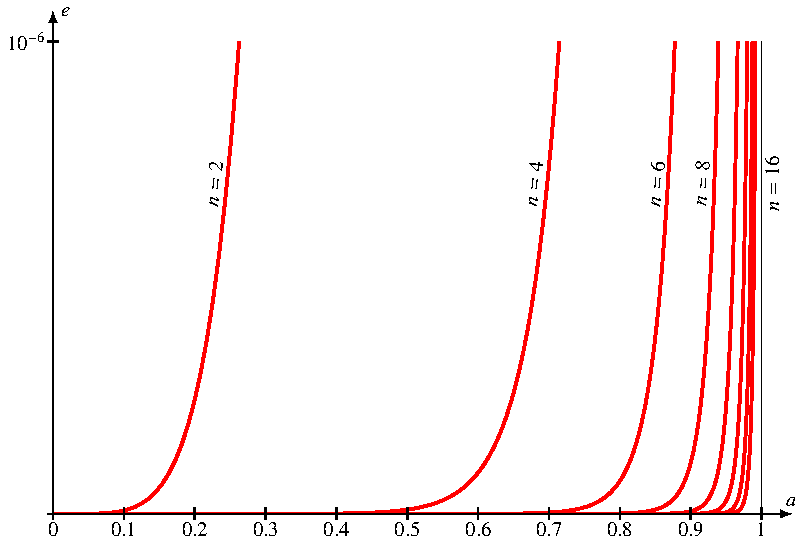
\includegraphics{chapters/060-integral/gq/gq.pdf}
\caption{Approximationsfehler des
Integrals~\eqref{buch:integral:gaussquadratur:bspintegral}
in Abhängigkeit von $a$.
Die Divergenz der Ableitung des Integranden an den Intervallenden
$\pm 1$ führt zu schlechter Konvergenz des Verfahrens, wenn $a$
nahe an $1$ ist.
\label{buch:integral:gaussquadratur:fehler}}
\end{figure}

Zur Illustration der Genauigkeit der Gauss-Quadratur berechnen wir
das Integral
\begin{equation}
\int_{-a}^a \sqrt{1-x^2}\,dx
=
\arcsin a + a \sqrt{1-a^2}
\label{buch:integral:gaussquadratur:bspintegral}
\end{equation}
mit Gauss-Quadratur einerseits und dem Trapezverfahren
andererseits.
Da Gauss-Quadratur mit sehr viel weniger Sützstellen auskommt,
berechnen wir die Trapeznäherung mit zehnmal so vielen Stützstelln.
In den Tabellen~\ref{buch:integral:gaussquadratur:table0.5}
und
\ref{buch:integral:gaussquadratur:table0.999}
sind die Resultate zusammengestellt.
Für $a =\frac12$ zeigt
Tabelle~\ref{buch:integral:gaussquadratur:table0.5}
die sehr schnelle Konvergenz der Gauss-Quadratur, schon mit
12 Stützstellen wird Maschinengenauigkeit erreicht.
Das Trapezverfahren dagegen erreicht auch mit 200 Stützstellen nur
4 korrekte Nachkommastellen.

An den Stellen $x=\pm 1$ divergiert die Ableitung des Integranden
des Integrals \eqref{buch:integral:gaussquadratur:bspintegral}.
Da grösste und kleinste Stützstelle der Gauss-Quadratur immer
deutlich vom Rand des Intervalls entfernt ist, kann das Verfahren
diese ``schwierigen'' Stellen nicht erkennen.
Tabelle~\ref{buch:integral:gaussquadratur:table0.999} zeigt, wie
die Konvergenz des Verfahrens in diesem Fall sehr viel schlechter ist.
Dies zeigt auch der Graph in
Abbildung~\ref{buch:integral:gaussquadratur:fehler}.

\subsection{Skalarprodukte mit Gewichtsfunktion}
Die Nullstellen der Legendre-Polynome ergaben ein gutes
Integrationsverfahren für Polynome auf einem beschränkten
Intervall.
Die Beispiele haben aber auch gezeigt, dass Stellen, wo die
Ableitung des Integranden divergiert, die Genauigkeit stark
beeinträchtigen können.
Ausserdem ist das Verfahren nicht anwendbar auf uneigentliche
Integrale.

\subsubsection{Umgang mit Singularitäten}
Die Lösung des Problems mit Stellen mit divergenter Ableitung
besteht darin, die Stützstellen in der Nähe dieser Stellen
zu konzentrieren.
Die Verwendung einer Gewichtsfunktion $w(x)$ kann genau dies
erreichen.
Statt das Integral einer Funktion $f(x)$ zu bestimmen, 
kann man $f(x)=g(x)w(x)$ schreiben, wobei $w(x)$ so
gewählt werden soll, dass das Verhalten der Steigung an
den Intervallenden gut wiedergibt.
Dies ist mit einer Jacobischen Gewichtsfunktion immer möglich.
Statt der Nullstellen der Legendre-Polynome sind dann die
Nullstellen der Jacobi-Polynome  und die Funktionswete von $g(x)$
an diesen Stellen zu verwenden,  die Gewichte sind
die Integrale von $l_i(x) P^{(\alpha,\beta)}(x)$.

\subsubsection{Uneigentliche Integrale}
Die Berechnung eines uneigentlichen Integrals auf dem Intervall
$(0,\infty)$ oder $(-\infty,\infty)$ ist aus mehreren Gründen nicht
direkt mit dem früher beschriebenen Gauss-Quadraturverfahren
möglich.

Die Stützstellen, die bei der Gauss-Quadratur in einem Intervall
$(a,b)$ verwendet werden, entstehen dadurch, dass man die Nullstellen
der Legendre-Polynome in $(-1,1)$ auf das Intervall $(a,b)$
skaliert.
Dies führt offensichtlich nicht zum Erfolg, wenn ein oder beide
Intervallgrenzen unendlich sind.
Dieses Problem kann dadurch gelöst werden, dass man das unendliche
Intervall $(a,\infty)$ mit
\[
x =  a + \frac{1-t}{t}
\]
auf das Intervall $[0,1]$ transformiert.

Will man beim Intervall $(0,\infty)$ bleiben, dann ist zu beachten,
dass das Integral eines Polynomes immer divergent ist, es ist also
auf jeden Fall nötig, den Integranden durch Funktionen zu approximieren,
die genügend schnell gegen $0$ gehen.
Polynome beliebigen Grades können verwendet werden, wenn sie mit
einer Funktion multipliziert werden, die schneller als jedes Polynom
gegen $0$ geht, so dass das Integral immer noch konvergiert.
Die Funktionen $e^{-x}$ für das Intervall $(0,\infty)$ oder
$e^{-x^2}$ für das Intervall $(-\infty,\infty)$ kommen dafür in Frage.

Um das Integral von $f(x)$ im Intervall $(0,\infty)$ zu berechnen,
schreibt man daher zunächst
\[
\int_0^\infty f(x)\,dx
=
\int_0^\infty g(x)e^{-x}\,dx
=
\int_0^\infty g(x) w(x)\,dx
\quad\text{mit}\quad
w(x)=e^{-x}
\text{ und }
g(x)=f(x)e^x.
\]
Dann approximiert $g(x)$ man durch ein Interpolationspolynom,
so wie man das bei der Gauss-Quadratur gemacht hat.
Als Stützstellen müssen dazu die Nullstellen der Laguerre-Polynome
verwendet werden.
Als Gewichte $w_i$ sind die Integrale der $l_i(x)e^{-x}$
zu verwenden.








\section*{Übungsaufgaben}
\rhead{Übungsaufgaben}
\aufgabetoplevel{chapters/060-integral/uebungsaufgaben}
\begin{uebungsaufgaben}
%\uebungsaufgabe{0}
%\uebungsaufgabe{1}
\end{uebungsaufgaben}

